\documentclass[a4paper,12pt,twoside]{../includes/ThesisStyle}
\usepackage[utf8]{inputenc}
\usepackage[T1]{fontenc}

\usepackage[left=1.5in,right=1.3in,top=1.1in,bottom=1.1in,includefoot,includehead,headheight=13.6pt]{geometry}\renewcommand{\baselinestretch}{1.05}


% =============================================================================
%\usepackage[sectionbib]{chapterbib}	% Cross-reference package (Natural BiB)
%\usepackage{bibunits}
%\usepackage{natbib}					% Put References at the end of each chapter
\usepackage{algorithm}
\usepackage{alltt}
\usepackage{amsfonts}
\usepackage{amsmath}
\usepackage{amssymb}
\usepackage{cite}
\usepackage{color}
\usepackage{enumerate}
\usepackage{booktabs} % used for \midrule
\usepackage{fancyhdr}					% Fancy Header and Footer
\usepackage{graphicx}
\usepackage{ifthen}
\usepackage{latexsym}
\usepackage{multirow}
\usepackage{rotating}					% Sideways of figures & tables
\usepackage{stmaryrd}
\usepackage{subfigure}
\usepackage{url}         
\usepackage{xspace}
\usepackage[normalem]{ulem} % for \sout
\usepackage{xcolor}
\usepackage{tablefootnote}
\usepackage{pifont}

% =============================================================================

% Table of contents for each chapter
\usepackage[nottoc, notlof, notlot]{tocbibind}
\usepackage{minitoc}
\setcounter{minitocdepth}{1}
\mtcindent=15pt

\setcounter{secnumdepth}{3}
\setcounter{tocdepth}{2}
  
% =============================================================================
% Fancy Header Style Options

\pagestyle{fancy}                       % Sets fancy header and footer
\fancyfoot{}                            % Delete current footer settings

%\renewcommand{\chaptermark}[1]{         % Lower Case Chapter marker style
%  \markboth{\chaptername\ \thechapter.\ #1}}{}} %

%\renewcommand{\sectionmark}[1]{         % Lower case Section marker style
%  \markright{\thesection.\ #1}}         %

\fancyhead[LE,RO]{\bfseries\thepage}    % Page number (boldface) in left on even
% pages and right on odd pages
\fancyhead[RE]{\bfseries\nouppercase{\leftmark}}      % Chapter in the right on even pages
\fancyhead[LO]{\bfseries\nouppercase{\rightmark}}     % Section in the left on odd pages

\let\headruleORIG\headrule
\renewcommand{\headrule}{\color{black} \headruleORIG}
\renewcommand{\headrulewidth}{1.0pt}
\usepackage{colortbl}
\arrayrulecolor{black}

\fancypagestyle{plain}{
  \fancyhead{}
  \fancyfoot{}
  \renewcommand{\headrulewidth}{0pt}
}


% =============================================================================
% Clear Header Style on the Last Empty Odd pages
\makeatletter

\def\cleardoublepage{\clearpage\if@twoside \ifodd\c@page\else%
  \hbox{}%
  \thispagestyle{empty}%              % Empty header styles
  \newpage%
  \if@twocolumn\hbox{}\newpage\fi\fi\fi}

\makeatother

\newenvironment{maxime}[1]
{
\vspace*{0cm}
\hfill
\begin{minipage}{0.5\textwidth}%
%\rule[0.5ex]{\textwidth}{0.1mm}\\%
\hrulefill $\:$ {\bf #1}\\
%\vspace*{-0.25cm}
\it 
}%
{%

\hrulefill
\vspace*{0.5cm}%
\end{minipage}
}

\let\minitocORIG\minitoc
\renewcommand{\minitoc}{\minitocORIG \vspace{1.5em}}


\renewcommand{\epsilon}{\varepsilon}

% centered page environment
\newenvironment{vcenterpage}
	{\newpage\vspace*{\fill}\thispagestyle{empty}\renewcommand{\headrulewidth}{0pt}}
	{\vspace*{\fill}}
	

%=============================================================================

\usepackage{needspace}
\newcommand{\needlines}[1]{\Needspace{#1\baselineskip}}

\usepackage{xcolor}
\definecolor{source}{gray}{0.95}
% source code formatting
\usepackage{listings}
    % global settings for source code listing package
\lstset{
    basicstyle=\ttfamily\small,
    showspaces=false,
    showstringspaces=false,
    captionpos=b, 
    columns=fullflexible}

\lstdefinelanguage{ST}{
    keywordsprefix=\#,
    morekeywords=[0]{true,false,nil},
    morekeywords=[1]{self,super,thisContext},
    morekeywords=[2]{ifTrue:,ifFalse:,whileTrue:,whileFalse:,and:,or:,xor:,not:,by:,timesRepeat:},
    sensitive=true,
    morecomment=[s]{"}{"},
    morestring=[d]',
    escapechar={!},
    alsoletter={., :, -, =, +, <},
    moredelim=**[is][\itshape]{/+}{+/},
    literate=
        {^}{{$\uparrow$}}1
        {:=}{{$\leftarrow$}}1
        {~}{{$\sim$}}1
        {-}{{\sf -\hspace{-0.13em}-}}1  % the goal is to make - the same width as +
        {+}{\raisebox{0.08ex}{+}}1		% and to raise + off the baseline to match V
        , % Don't forget the comma at the end!
    style=STStyle
}
\lstdefinestyle{STStyle}{
    tabsize=4,
    %frame=leftline,
    % frame=bl,
    %framerule=2pt,
    %rulecolor=\color{gray},
    % backgroundcolor=\color{white},
    %backgroundcolor=\usebeamercolor[bg]{listing},
    basicstyle=\ttfamily\small,
    keywordstyle=\bf\ttfamily,
    % stringstyle=\color{orange},
    stringstyle=\mdseries\slshape,
    commentstyle=\it\rmfamily\color{darkgray}, 
    commentstyle=\mdseries\slshape\color{gray},
    %commentstyle=\mdseries\slshape,
    emphstyle=\bf\ttfamily,
    escapeinside={!}{!},
	%backgroundcolor=\color{source},
    %emphstyle={[2]\color{red}},
    %emphstyle={[3]\color{blue}\bf},
    %emphstyle={[4]\color{blue}},
    keepspaces=true
} 

%\lstnewenvironment{javacode}  [1][]{\lstset{language=java,#1}\needlines{#2}}{} 
%\lstnewenvironment{pythoncode}[2][]{\lstset{language=python,#1}\needlines{#2}}{}
\lstnewenvironment{stcode}    [2][]{\lstset{language=ST,#1}\needlines{#2}}{}
\lstnewenvironment{ccode}     [2][]
    {\lstset{language=C,numbers=left,escapechar=\$,numberstyle=\tiny,#1}\needlines{#2}}{}

% ON: I tried to pass the line number options in as arg #1 but it does not work for me
% I also could net get the line numbers to consistently increase
\lstnewenvironment{numstcode} [2][]
    {\lstset{language=ST,numbers=left,numberstyle=\tiny,numbersep=2pt,#1}\needlines{#2}}{}
\lstnewenvironment{numstcodecont} [2][]
    {\lstset{language=ST,numbers=left,numberstyle=\tiny,numbersep=2pt,firstnumber=last#1}\needlines{#2}}{}

\newcommand{\lst}[1]{{\tt #1}}

% In-line code (literal)

% In-line code (latex enabled)
% Use this only in special situations where \ct does not work
% (within Section headings ...):
\newcommand{\lct}[1]{{\textsf{\textup{#1}}}}
% Code environments
\lstnewenvironment{code}{%
	\lstset{%
		% frame=lines,
		frame=single,
		framerule=0pt,
		mathescape=false
	}
}{}

%\renewcommand{\lstlistingname}{Code Example}

% =============================================================================
\newboolean{showcomments}
\setboolean{showcomments}{true}

\ifthenelse{\boolean{showcomments}} {
	\newcommand{\ugh}[1] {\textcolor{red}{\uwave{#1}}}	% please rephrase
	\newcommand{\ins}[1] {\textcolor{blue}{\uline{#1}}}	% please insert
	\newcommand{\del}[1] {\textcolor{red}{\sout{#1}}}	% please delete
	\newcommand{\chg}[2] {								% please change
		\textcolor{red}{\sout{#1}}{\ra}
		\textcolor{blue}{\uline{#2}}}
	\newcommand{\nbc}[3]{								% comment
		{\colorbox{#3}{\bfseries\sffamily\scriptsize\textcolor{white}{#1}}}
		{\textcolor{#3}{\sf\small$\blacktriangleright$\textit{#2}$\blacktriangleleft$}}}

}{
	\newcommand{\ugh}[1]{#1}							% please rephrase
	\newcommand{\ins}[1]{#1}							% please insert
	\newcommand{\del}[1]{}								% please delete
	\newcommand{\chg}[2]{#2}							% please change
	\newcommand{\nbc}[3]{}								% comment
}

% =============================================================================
\usepackage[pagebackref,hyperindex=true]{hyperref}


% Links in pdf
\usepackage{color}
\definecolor{linkcol}{rgb}{0.0, 0.0, 0.0} 
\definecolor{citecol}{rgb}{0.0, 0.0, 0.0} 

% Change this to change the informations included in the pdf file
% See hyperref documentation for information on those parameters
\hypersetup {
	bookmarksopen=true,
	pdftitle="Design and Use of Anatomical Atlases for Radiotherapy",
	pdfauthor="Olivier COMMOWICK", 
	pdfsubject="Creation of atlases and atlas based segmentation", %subject of the document
	%pdftoolbar=false, % toolbar hidden
	pdfmenubar=true, %menubar shown
	pdfhighlight=/O, %effect of clicking on a link
	colorlinks=true,
	pdfpagemode=UseNone,
	pdfpagelayout=SinglePage,
	pdffitwindow=true,
	linkcolor=linkcol,
	citecolor=citecol,
	urlcolor=linkcol
}

% =============================================================================
\newcommand{\figlabel}[1] {\label{fig:#1}}
\newcommand{\chaplabel}[1]{\label{chap:#1}}
\newcommand{\seclabel}[1] {\label{sec:#1}}
\newcommand{\tablabel}[1] {\label{tab:#1}}
\newcommand{\lstlabel}[1] {\label{lst:#1}}

\newcommand{\figref}[1] {Figure~\ref{fig:#1}}
\newcommand{\chapref}[1]{Chapter~\ref{sec:#1}}
\newcommand{\secref}[1] {Section~\ref{sec:#1}}
\newcommand{\tabref}[1] {Table~\ref{tab:#1}}
\newcommand{\lstref}[1] {Listing~\ref{tab:#1}}

\newcommand{\commented}[1]{}

\newcommand{\bs}    {\symbol{'134}} % backslash
\newcommand{\us}    {\symbol{'137}} % underscore
\newcommand{\ttt}[1]{\texttt{#1}}
\newcommand{\ie}    {\emph{i.e.},\xspace}
\newcommand{\eg}    {\emph{e.g.},\xspace}
\newcommand{\etal}  {\emph{et al.}\xspace}
\newcommand{\ns}    {\!\!\!\!} %big negative space
\newcommand{\cnull} {\textbackslash0\xspace}


\newcommand\fix[1]{\nb{FIX}{#1}}
\newcommand\todo[1]{\nb{TO DO}{#1}}
\newcommand\cb[1]{\nbc{CB}{#1}{purple}}
\newcommand\sd[1]{\nbc{SD}{#1}{orange}}
\newcommand\is[1]{\nbc{IS}{#1}{gray}}
\newcommand\gc[1]{\nbc{GC}{#1}{olive}}
\newcommand\ct[1]{\nbc{CT}{#1}{teal}}
\newcommand\md[1]{\nbc{MD}{#1}{blue}}
\newcommand\dc[1]{\nbc{DC}{#1}{green}}

% =============================================================================
\newcommand{\NBFFI}  {Native\-Boost-FFI\xspace}
\newcommand{\NB}  {Native\-Boost\xspace}
\newcommand{\B}   {Benzo\xspace}
\newcommand{\ST}  {Small\-talk\xspace}
\newcommand{\PH}  {Pharo\xspace}
\graphicspath{{.}{../figures/}}

\begin{document}
% ===========================================================================
\chapter{\B: Low-level Glue in \PH}
\chaplabel{benzo}
\minitoc
% ===========================================================================
\introduction
% ===========================================================================

In this chapter we present \B a framework that connects the low-level / \VM work with a reflective and dynamic language-side library.
Unlike more classical approaches \B does not resort to vast set of customized \VM primitives or plugins.
Instead it relies on a generic primitive to activated native code that is generated at language-side.

\B provides a unique experience of being extremely low-level yet using high-level concepts at the same time.
This is possible since the framework is implemented at language-side and tightly integrated into the \PH development environment.
In this chapter we present in detail how \B interacts with \PH and what the difficulties are.
The key components of \B are:
\begin{itemize}[noitemsep]
\item A generic primitive to activate native code
\item \AsmJIT A language-side assembler
\item A language-side library for installing and activating native code
\end{itemize}

\noindent Based on \B we outline 3 unique applications in \secref{benzo-usecase}:
\begin{itemize}[noitemsep]
\item Foreign Function Interfaces (in more detail in \chapref{ffi})
\item Dynamic Primitives (in more detail in  \chapref{validation})
\item Language-side \JIT (in more detail in  \chapref{validation})
\end{itemize}


% ===========================================================================
\newpage
\section{Background}
\seclabel{benzo-background}
% ===========================================================================
High-level low-level programming \cite{Fram09a} encourages to use high-level languages such as \Java to build low-level execution infrastructures or to do system programming. 
It is successfully used in experimental high-level self-hosted virtual machines (\VMs) such as \Jikes~\cite{Alpe99a}.  
Frampton et al. present a framework that is biased towards a statically typed high-level language, taking strict security aspects into account.
Their approach promotes to address low-level system programming tasks with the tools and abstractions of high-level languages.
However, their solution has reduced applicability in a dynamic and reflective context.
By reflective, we refer to the combined capabilities to inspect (introspection) and change (intercession) the same execution concepts at runtime \cite{Maes87a}.

From a reflective point of view it seems natural to dynamically modify the \VM at runtime and not just at compile-time.
If we are able to modify the \VM from language-side we blur the line between these two distinct worlds, becoming indistinguishable to talk about the \VM or the language-side.
Hence throughout this chapter we use the term language runtime to refer to the running \VM combined with the language-side application.


% ---------------------------------------------------------------------------
\subsection{Requirements}
% ---------------------------------------------------------------------------

Extending the \VM is only one particular case of modifying or extending the complete language runtime.
Language-side libraries, reflective capabilities, \VM extensions or hybrid approaches are other possibilities which we discuss in detail in \secref{benzo-related}.
All these typical extension mechanisms are not sufficient if we want to modify the \VM from language-side, or in our terminology, to reflectively modify the language runtime. Furthermore these mechanisms are based on the fact that there is a clear barrier between language and \VM.
A solution that crosses these barriers requires the following properties:

\begin{enumerate}
	\item It must be \emph{reflective} in the sense it must support \emph{dynamic} changes of the language runtime (\VM) without requiring a system restart.
	\item It should imply minimal changes to the existing low-level runtime to \emph{considerably reduce development efforts}.
\end{enumerate}


% ---------------------------------------------------------------------------
\subsection{\B a Framework for Reflective Low-level Programming}
% ---------------------------------------------------------------------------

High-level low-level programming is a powerful technique for system programming without resorting to static low-level environments \cite{Fram09a,Wimm13a} that almost fulfills our requirements.
However, in a reflective setup it fails to comply with the first requirement mentioned in the previous paragraph: it does not allow reflective changes at runtime.
Our approach for overcoming this limitation consists of \B, a lightweight and reflective framework that dynamically generates native code from language-side and allows its execution on the fly.
It relies only on a small set of generic \VM extensions described in \secref{benzo-vm-requirements}, whereas the vast majority of the framework is implemented as a language-side library.

% ---------------------------------------------------------------------------
\subsection{\B Applications}
% ---------------------------------------------------------------------------
In \secref{benzo-usecase} we advocate the contribution of \B by providing three different incremental examples that heavily use the framework.
Unlike typical implementations that would focus on writing them as \VM extensions, we implement them completely at language-side using \B:

\begin{description}
	\item[Language-side \FFI] A complete language-side Foreign Function Interface (\FFI) implementation, described in \secref{benzo-ffi} and in more detail in \chapref{ffi}.
	\item[Dynamic Primitives] A language-side compilation toolchain that replaces system primitives at runtime with customized code, described in \secref{benzo-waterfall} and in more detail in \secref{val-waterfall}. 
	\item[Language-side \JIT Compiler] A \JIT compiler that works at language-side and interacts with the \VM for code synchronization, described in \secref{benzo-nabujito} and in more detail in \secref{val-nabujito}.
\end{description}

\noindent Illustrated by these three distinct examples, the contributions of this chapter are:
\begin{enumerate} 
	\item A \emph{reflective} high-level low-level programming framework that encourages the extension of high-level language runtimes on the fly without the overheads imposed by pure high-level solutions. 
	\item A proof of concept of the proposal with the implementation and description of three different tools that heavily use reflective low-level programming and covers distinct scenarios.
\end{enumerate}

% ===========================================================================
\section{The \B Framework}
\seclabel{benzo-benzo}
% ===========================================================================
\B is implemented in \urlfootnote{\PH}{http://pharo.org/}, a \ST inspired language.
\PH comes with all the reflective capabilities known from \ST where most language-side components can be altered dynamically.
\B is implemented at language-side and only requires the help of two simple and generic primitives to activate native code and resolve the entry point address position of referenced C functions.

%----------------------------------------------------------------------------
\subsection{\VM Context}
\seclabel{benzo-vm-requirements}
%----------------------------------------------------------------------------
\PH emerged from the Squeak project \cite{Inga97a}.
The \PH \VM (Cog) implementation \cite{Mira11a} also evolved from the original Squeak bytecode interpreter.
The current \VM uses a moving Garbage Collector (\GC) with two generations\gc{ref?} and uses a \JIT that applies basic register allocation to reduce stack load. 
This situation is not a direct requirement for \B but it is assumed as given and thus not further discussed in detail.
However, \B requires certain features that were not supported in the existing \VM implementation.
Mainly our requirement is being able to generate executable code and activate it at runtime.
This is general and essential so it applies to any \VM that wants to support dynamic code execution managed at language-side.

%----------------------------------------------------------------------------
\paragraph{Executable Memory.}
\seclabel{benzo-exeutable-memory}
 
We chose to follow a very lightweight approach to dynamically execute native code at runtime. 
Since we use \PH as our host language it is a natural choice to manage the native code at language-side and use as little VM features as possible.
Hence we use normal \PH objects to hold the generated native code.

However, by default the object memory is not executable.
This leaves two choices, either mark the whole object memory executable or move the objects with the native code to a special executable memory region.
We took the path of least resistance and marked the whole object memory as executable.
The other solution requires substantial changes for memory management. 

The \GC of the \PH \VM uses a moving semi-space approach with two generations.
Additionally there is a fixed sized executable region used for the \JIT as a buffer for runtime generated native code.
The \JIT space uses its own small garbage collection strategy which is decoupled from the rest of the object memory.
This also means that the \JIT space does not hold normal \PH objects but special low-level structures.
As mentioned before, the \JIT space is limited in size and eventually fills up, causing the \JIT to spill older code structures from there. 

All in all the \JIT-space does not seem to be the right place for storing persistent \PH objects holding native code.
Instead we opt for the completely executable object memory option and store all the executable code in standard \PH objects.
As the \VM has a moving \GC, it gives us certain restrictions on what kind of native code we can run directly from the language-side. 
As we will describe in \secref{benzo-platform-interaction}, we can access high-level \PH objects only via an indirection from low-level code.

%----------------------------------------------------------------------------
\paragraph{\VM Interaction.}
\seclabel{benzo-vm-interaction}

The standard way in \PH to execute low-level code is to use a tag in the method definition. The following example shows such a method on the \ttt{Float} class.
%
\begin{stcode}[label={lst:benzo-basic-primitive}]{5}
* aNumber 
	<primitive: 49>
	^ aNumber adaptToFloat: self andSend: #*
\end{stcode}
%
Here we use the primitive 49 to call a \VM function which efficiently multiplies two floats. 
\figref{benzo-smalltalkPrimitive}-a describes the case where the primitive is successfully executed.
However, if the primitive is unable to do the operation, for instance if the argument \ttt{aNumber} is not a float, it will signal a failure which causes the \VM to execute the fallback \PH code in the method body.  
\figref{benzo-smalltalkPrimitive}-b describes it. 
In the floating point multiplication example the fallback code uses a slow conversion method to polymorphically convert other objects to floats and defer the multiplication.


\begin{figure}[ht]
	\centering
	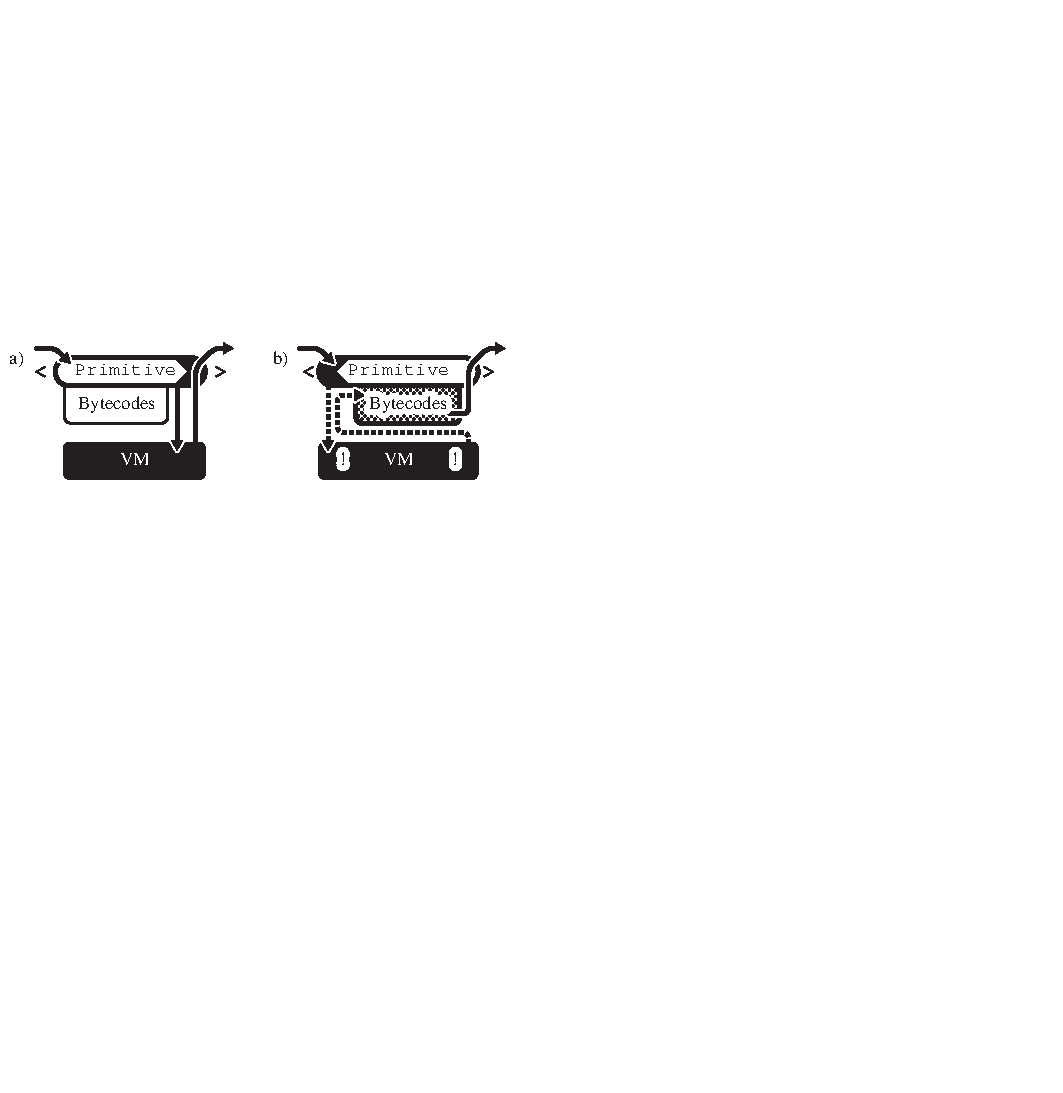
\includegraphics[scale=1.1]{smalltalkPrimitive}
	\caption[\PH Primitive]{Generic primitive methods in \PH: a) A primitive completely bypasses the bytecode, b) A failing primitive executes the bytecode as fallback.}
	\figlabel{benzo-smalltalkPrimitive}
\end{figure}

\noindent \B uses the primitives as a gate to enter the low-level world from the language-side.
Our custom primitive then executes the generated native code and returns to language-side. 
This code is appended inside the compiled method object.
When the primitive is activated, it  accesses the currently executed compiled method via a \VM function. 
\figref{benzo-nativeCodeMethod} shows the structure of a \PH compiled method that has native code attached to it.
We see the primitive tag on top, followed by the literal frame which holds references to symbols and classes used in the method.
The subsequent \PH bytecode is the fallback code executed only if the primitive fails. Only then appears the native instructions.
A marker at the end of the compiled method called trailer type is used to flag methods that actually have native code attached to them.
%
\begin{figure}[ht]
	\centering
	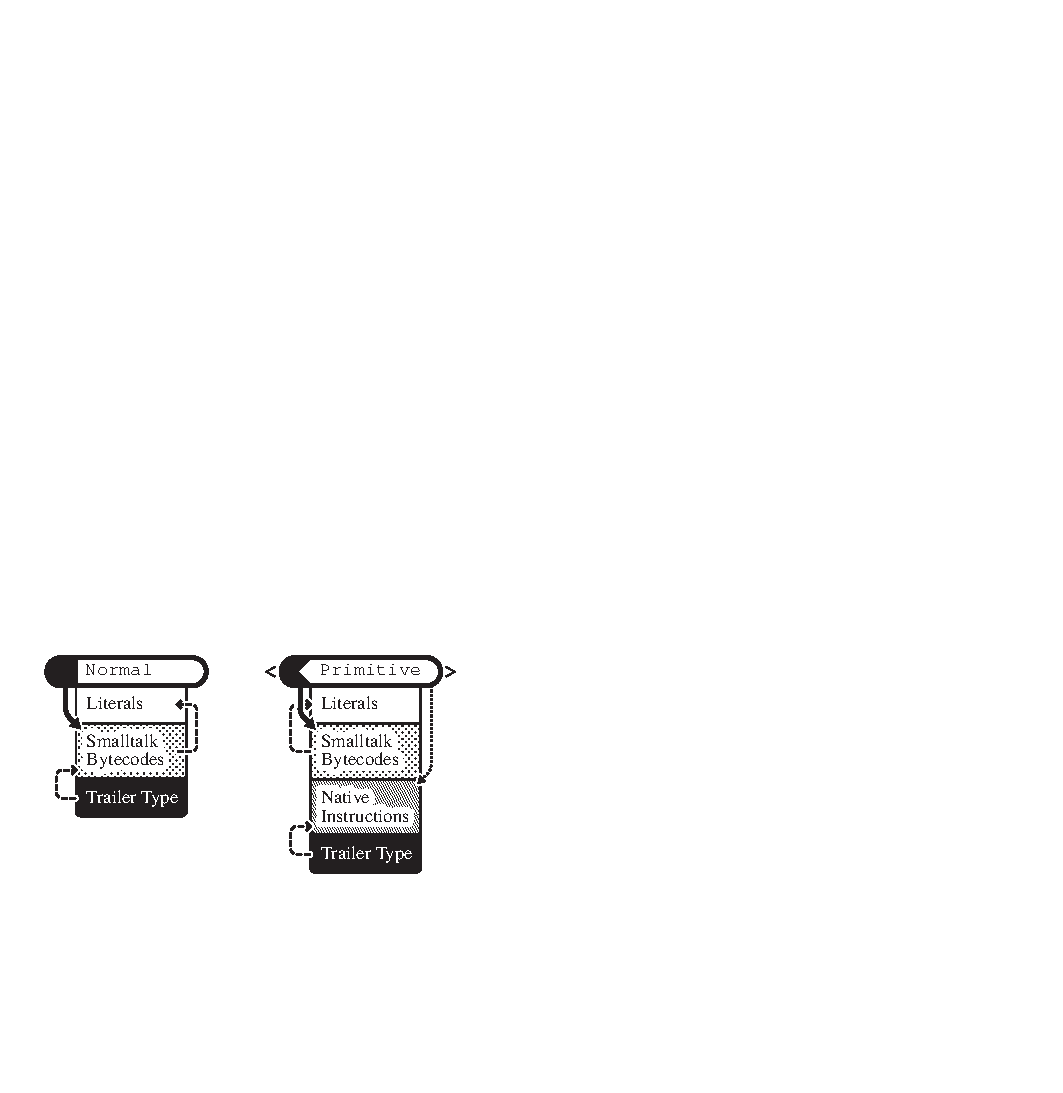
\includegraphics[scale=1.1]{nativeCodeMethod}
	\caption[\PH Compiled Method]{A standard \PH compiled method on the left and a method with appended native instructions generated by \B.}
	\figlabel{benzo-nativeCodeMethod}
\end{figure}

\noindent Since compiled methods are first-class objects it is possible to modify them at runtime and append the native code.
The primitive \ttt{primitiveNativeCall}, which is implemented by \B, is the responsible of running the native instructions in a \PH method.
The code example \ttt{interrupt3} shows a very basic application of our infrastructure.
%
\begin{stcode}[label={lst:benzo-basic-native-code}, caption={\PH method using \B for very basic low-level debugging.}, escapeinside={@}{@}]{5}
interrupt3
	<primitive: 'primitiveNativeCall' 
	 module: 'Benzo' >
	Benzo generate: [ :asm | asm int3 ]
\end{stcode}
%
The primitive named \ttt{primitiveNativeCall} on the first line tries to run the native instructions appended to the compiled method.
When there is no native code yet the primitive fails and on return it evaluate the rest of the \PH code in the method.
In \secref{benzo-language-side}, through more detailed examples, we describe how \B uses \PH code to generate the native instructions
Figure \figref{nativeCodeMethodDetail} shows the resulting compiled method in full detail..
%
\begin{figure}[ht]
    \centering
    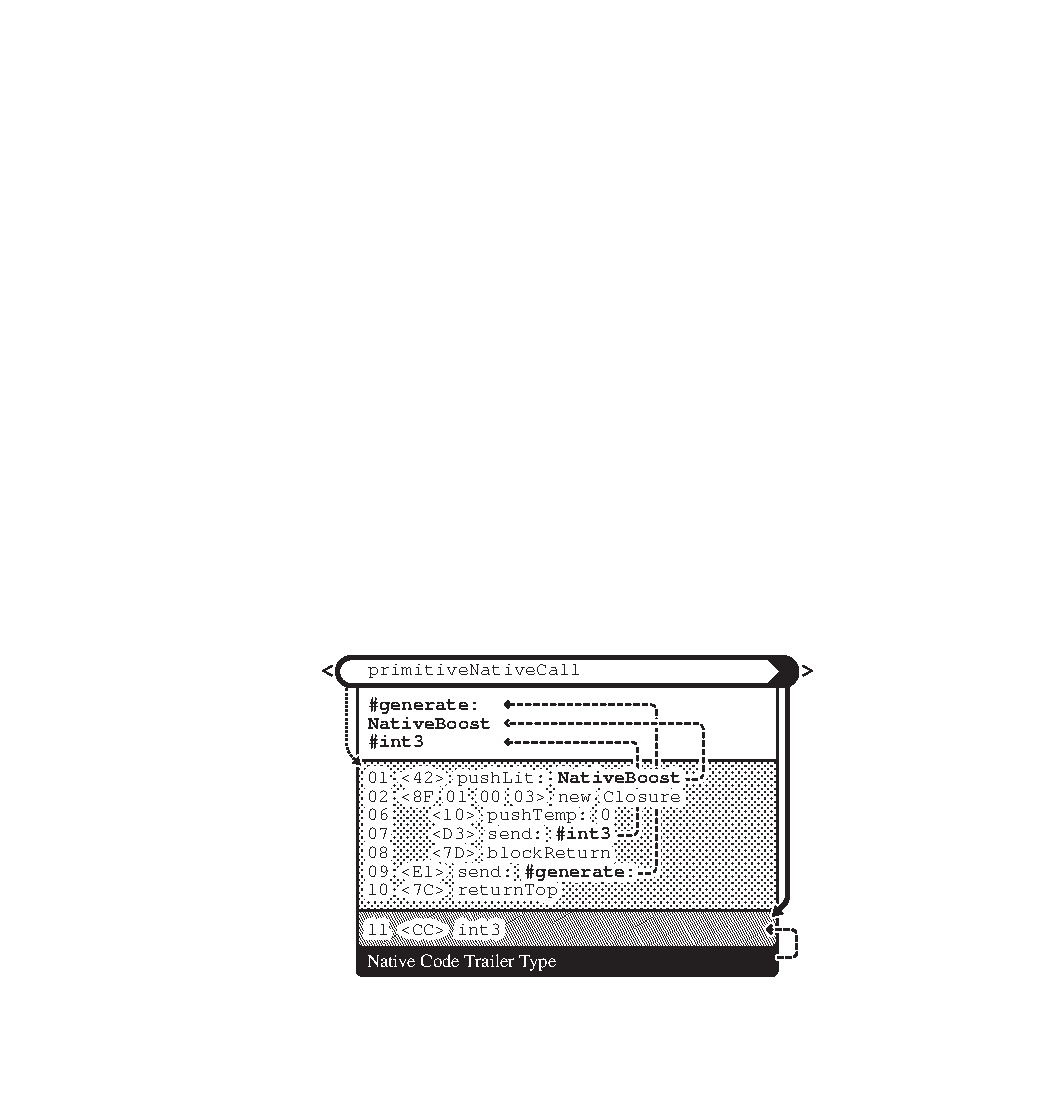
\includegraphics[scale=1.1]{nativeCodeMethodDetail}
    \caption[\ttt{CompiledMethod} With \B Code]{Example of \PH method with native code which calls the low-level debug exception handler \ttt{INT3}. The bytecode references objects indirectly via the literal frame residing at the beginning of the method.}
    \figlabel{nativeCodeMethodDetail}
\end{figure}

%----------------------------------------------------------------------------
\paragraph{Native Code Platform Interaction.}
\seclabel{benzo-platform-interaction}

To ensure that the code is compatible with the current platform a \VM specific marker is expected at the beginning of the native code on the compiled method.
Upon activation \B compares this marker with the one from the current \VM.
If they don't match, \B signals a failure that causes the \VM to evaluate the fallback \PH code.
With this elegant approach \B regenerates native code lazily on new platforms.
Moreover, it does not have to flush the native code when the application is restarted on the same platform.

%----------------------------------------------------------------------------
\paragraph{Garbage Collector Interaction.}
\seclabel{benzo-gc-interaction}

Compiled methods in \PH have a special section, the literal frame, which stores objects referenced in the bytecodes.
Bytecodes then only have indirect access to these objects by indexing into the literal frame.
This simplifies the implementation of the garbage collector as it only has to scan the beginning of each method for possible references to objects. 
So the \GC only tracks \PH objects when they are in the method literal frame. 
The moving \GC of the \VM used for \PH has a significant impact on the low-level code we can generate using \B.
For instance it is not possible to statically refer to language-side objects from native code as object addresses change after each garbage collection.
Modifying the \GC to support regions of non-moving objects would solve this problem.
However, we chose to minimize the number of low-level \VM modification necessary to run our experiments and opted for a simpler solution.

\begin{figure}[ht]
	\centering
	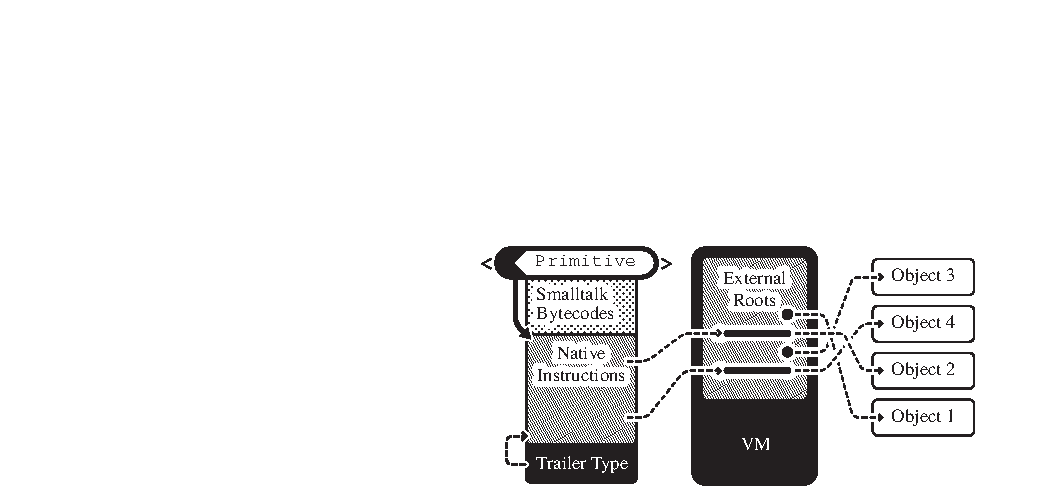
\includegraphics[scale=1.1]{externalRoots}
	\caption[Benzo External Roots]{Pointers to objects registered as external roots are pinpointed at fixed offset in global \VM-level object.
	}
	\figlabel{benzo-externalRoots}
\end{figure}

\noindent \B accesses language-side objects through an indirection.
For indirectly accessing objects the \PH \VM already features a special structure, named \emph{external roots}.
This array has a fixed-location in memory which can be used to access moving language-side objects.
The \GC updates the addresses in this \VM structure after each run.
Hence we have the static address of the external roots object as an entry point to statically access \PH objects.
Summarizing, for accessing \PH objects within native code we first register it as an external root object and access it only indirectly.
This means that for native code, instead of a method-local literal array we share a global literal array as shown in \figref{benzo-externalRoots}. 
\B only adds an \ttt{Array} to the external root objects which is managed from language-side and administers all references.

%\revc{The external roots concept appears here first but the idea of "indirection" has been mentioned. The regular literal frame of compiled methods are discussed heavily; that would suggest that the generated native code could use relative offset from the code location and still be able to "pin-point" the literal slot in the literal frame. What is the downside of this approach? (And how slots in the external roots garbage collected?)}
%\gc{I'm not very interested with the comment above. But perhaps here it is a good place to say that once the native code start executing our \VM assures that a \GC could not happen}
%----------------------------------------------------------------------------
\paragraph{\JIT Interaction.}
\seclabel{benzo-jit-interaction}

A special case worth being mentioned is the interaction of \B and the JIT.
When the \PH \VM starts the execution of dynamic generated code the execution environment changes slightly.
Similarly, when entering primitives or plugin code, the managed execution mode is left and a normal C-level execution environment is reestablished until the primitive finishes and the \VM jumps back to the jitted code.
These context switches impose an overhead and can be avoided in the case of calling native code.
For this reason we extend the \VM to support inlining of native code in the \JIT phase following the same strategy as other existing primitives which are inlined at \JIT-level.
%
\begin{figure}[ht]
	\centering
	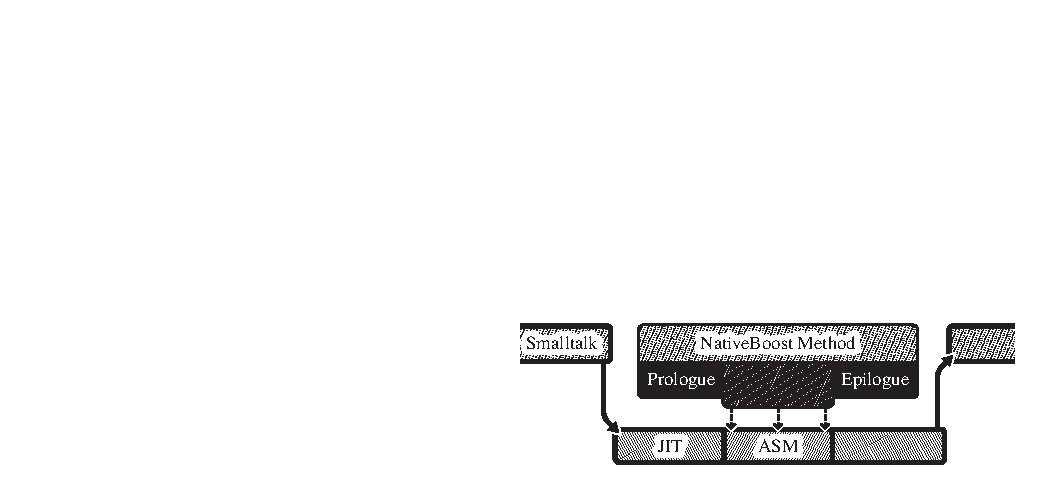
\includegraphics[scale=1.1]{nabujitoInline}
	\caption[\B \JIT Interaction]{\B inlining language-side native code into jitted mode.}
	\figlabel{benzo-nabujitoInline}
\end{figure}
%
\figref{benzo-nabujitoInline} shows how the native code from a \B enabled method is inlined into the JIT infrastructure.
The \B prologue and epilogue used for managing the low-level stack are replaced by an adapted version for the JIT.
The performance boost of this optimization is further discussed in \secref{benzo-issues-performance}.


%----------------------------------------------------------------------------
\paragraph{Error Handling.}
\seclabel{benzo-error-handling}

\B provides an error handling facility that allows to return high-level error messages from the low-level code.
The native code builder provides a helper method called \ttt{failWithMessage:} that generates the proper assembler instructions to return a full error message. The following code shows an example application of this behavior.
%
\begin{stcode}[emph={asm}]{5}
failWithErrorMessage
	<primitive: 'primitiveNativeCall' 
	 module: 'Benzo' >
	 Benzo x86 generate: [ :asm :helper |
		helper failWithMessage: 'Value is not 0'.].
\end{stcode}
%
Under the hood, \B reuses the existing built-in error mechanism of \PH primitives.
However, primitives only allow for error number to be returned which limits the expressiveness of the error messages.
To circumvent this limitation \B assigns a unique error number for each error message pass to \ttt{failWithMessage:}.
The mapping between the two error message representation, its error number and the message string itself, happens at language-side.
\B simply reuses the existing infrastructure to improve the debugging tasks and promote a better interaction with developers.

%----------------------------------------------------------------------------
\subsection{\B's Language-Side Implementation}
\seclabel{benzo-language-side}
%----------------------------------------------------------------------------
As a key design decision, we determine to keep the interface to the low-level world minimal.
The following describes the features of \B at the high-level language-side.

%----------------------------------------------------------------------------
\paragraph{Code Generation.}
\seclabel{benzo-code-generation}

\B delegates native code generation to a full assembler written in \PH. The following example shows how to use the assembler to generate the native code for moving \ttt{1} into the 32-bit register \ttt{EAX}.
%
\begin{stcode}{4}
Benzo x86 generate: [ :asm |
	asm mov: 1 asUImm to: asm EAX ].
\end{stcode}
%
The implementation first creates a slightly more abstract intermediate format.
The abstract operations can be extended by custom operations that may expand to several native instructions. For pragmatic reasons current implementation only supports \textsc{x86} and \textsc{x86-64}.
The full features of the high-level environment are available when generating native code.
Hence complex instruction sequences can easily be delegated to other objects.
In the following example we use a \VM helper to instantiate an array. It is worth noting that all are standard message sends:
%
\begin{stcode}{5}
Benzo x86 generate: [ :asm :helper | | register |
	register := helper classArray.
	register := helper 
		instantiateClass: register
		indexableSize: 10
	asm mov: register to: asm resultRegister ].
\end{stcode}
%
The \VM helper exposes a basic, low-level interface to access objects and its properties.
Additional methods cover the access to the external roots described in \secref{benzo-gc-interaction}.
In this case the \ttt{\#instantiateClass:indexableSize:} will generate the proper native code to call to a \VM function and make sure that the side-effects of a possible \GC run are handled properly.
By default the value in the result register is returned back to the language-side. On \textsc{x86} this defaults to \ttt{EAX}.
In \secref{benzo-usecase} we introduce more substantial applications based on \B.

%----------------------------------------------------------------------------
\paragraph{Code Activation.}
\seclabel{benzo-code-activation}
 
So far we only broadly described how \B activates the native code.
In a nutshell, we generate native code using our own language-side assembler and then we attach the native instructions to compiled methods as shown in figure \figref{nativeCodeMethodDetail}.
Additionally we mark the method to use a primitive defined \B plugin.
The \B primitive is responsible for the native code activation which consists of three main steps:
%
\begin{enumerate}[noitemsep]
	\item Check if there is native code in the actual compiled method and if it is compatible with the current platform.
	\item Generate native code if necessary.
	\item Activate the native code for execution.
\end{enumerate}

\noindent The first time a method with \B-based native code is activated the linked \B primitive will fail and run the normal \PH code in this method (see \secref{benzo-vm-interaction}).
This is where the actual native code generation happens.
As shown in previous examples, the native code is expressed in standard \PH code using our language-side assembler.
Once the whole code is generated, it is appended to the compiled method body leaving the existing \PH bytecodes intact.
Behind the scenes \B adds some more information to the code as the previously mentioned platform marker. 

\begin{figure}[ht]
	\centering
	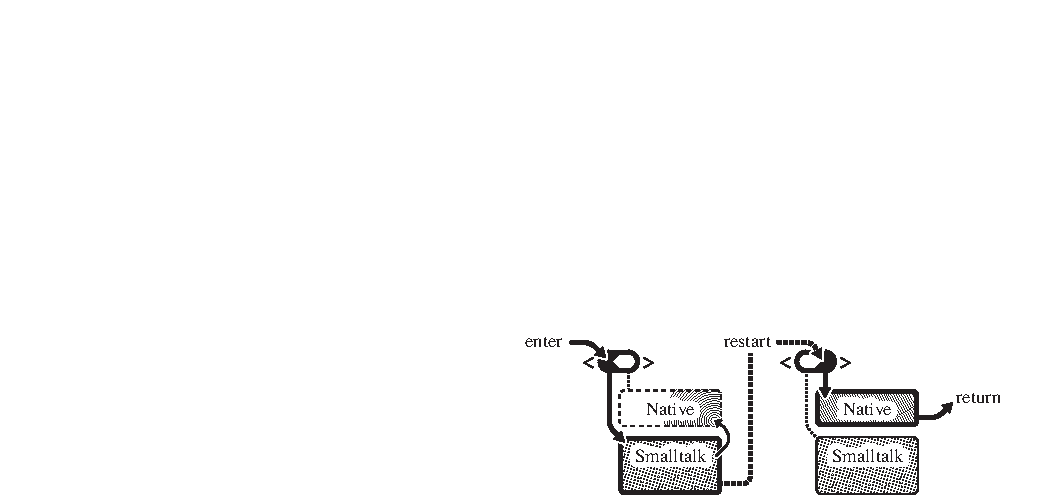
\includegraphics[scale=1.1]{nativeCodeActivation}
	\caption[\B Native Code Acivation]{Native code activation with \B: The first call triggers the code generation. Then the method is restarted and the native code executed.}
	\figlabel{benzo-nativeCodeActivation}
\end{figure}

\noindent Now we completed the first the left half of the activation process shown in \figref{benzo-nativeCodeActivation}.
What is left is the third step, the actual activation of the native code.
After we the native code is installed in the compiled method, we still run \PH code to restart the same \B-enabled method again, this corresponds to the arrow in \figref{benzo-nativeCodeActivation} connecting both sides.
For activation \B uses reflective features to restart the method.
Imagine that the method takes some arguments.
These arguments have to be preserved during the code-generation phase and reused for the second activation.
\B will simply use \PH's reflective \ttt{\#perform:withArguments:} method on the original receiver to restart/activate the same method with the same arguments again.

When running the \B-enabled method again the \B primitive is activated once more.
However, this time native code is present and thus the \B jumps to code attached to the compiled method and returns the generated result.
This is depicted in the right half of \figref{benzo-nativeCodeActivation}.

% ===========================================================================
\section{\B in Practice}
\seclabel{benzo-usecase}
% ===========================================================================
In this section we present the outline 3 distinct solutions built on top of \B: A \FFI, dynamic primitives and a \JIT (\chapref{ffi} and \chapref{validation} provide more detailed insight).
Typically these implementations would require a custom-tailored \VM or specialized plugins.
However, we show that it is possible to implement them using the generic functionality provided by \B.

The chosen application, starting with the \FFI, are increasingly more \VM bound.
Whereas the typical \FFI implementation is based on an separate plugin, dynamic primitives or a \JIT require persistent changes in the underlying \VM.


%----------------------------------------------------------------------------
\subsection{\NB: \B-based Foreign Function Interface}
\seclabel{benzo-ffi}
%----------------------------------------------------------------------------

\begin{figure}[h]
	\centering
	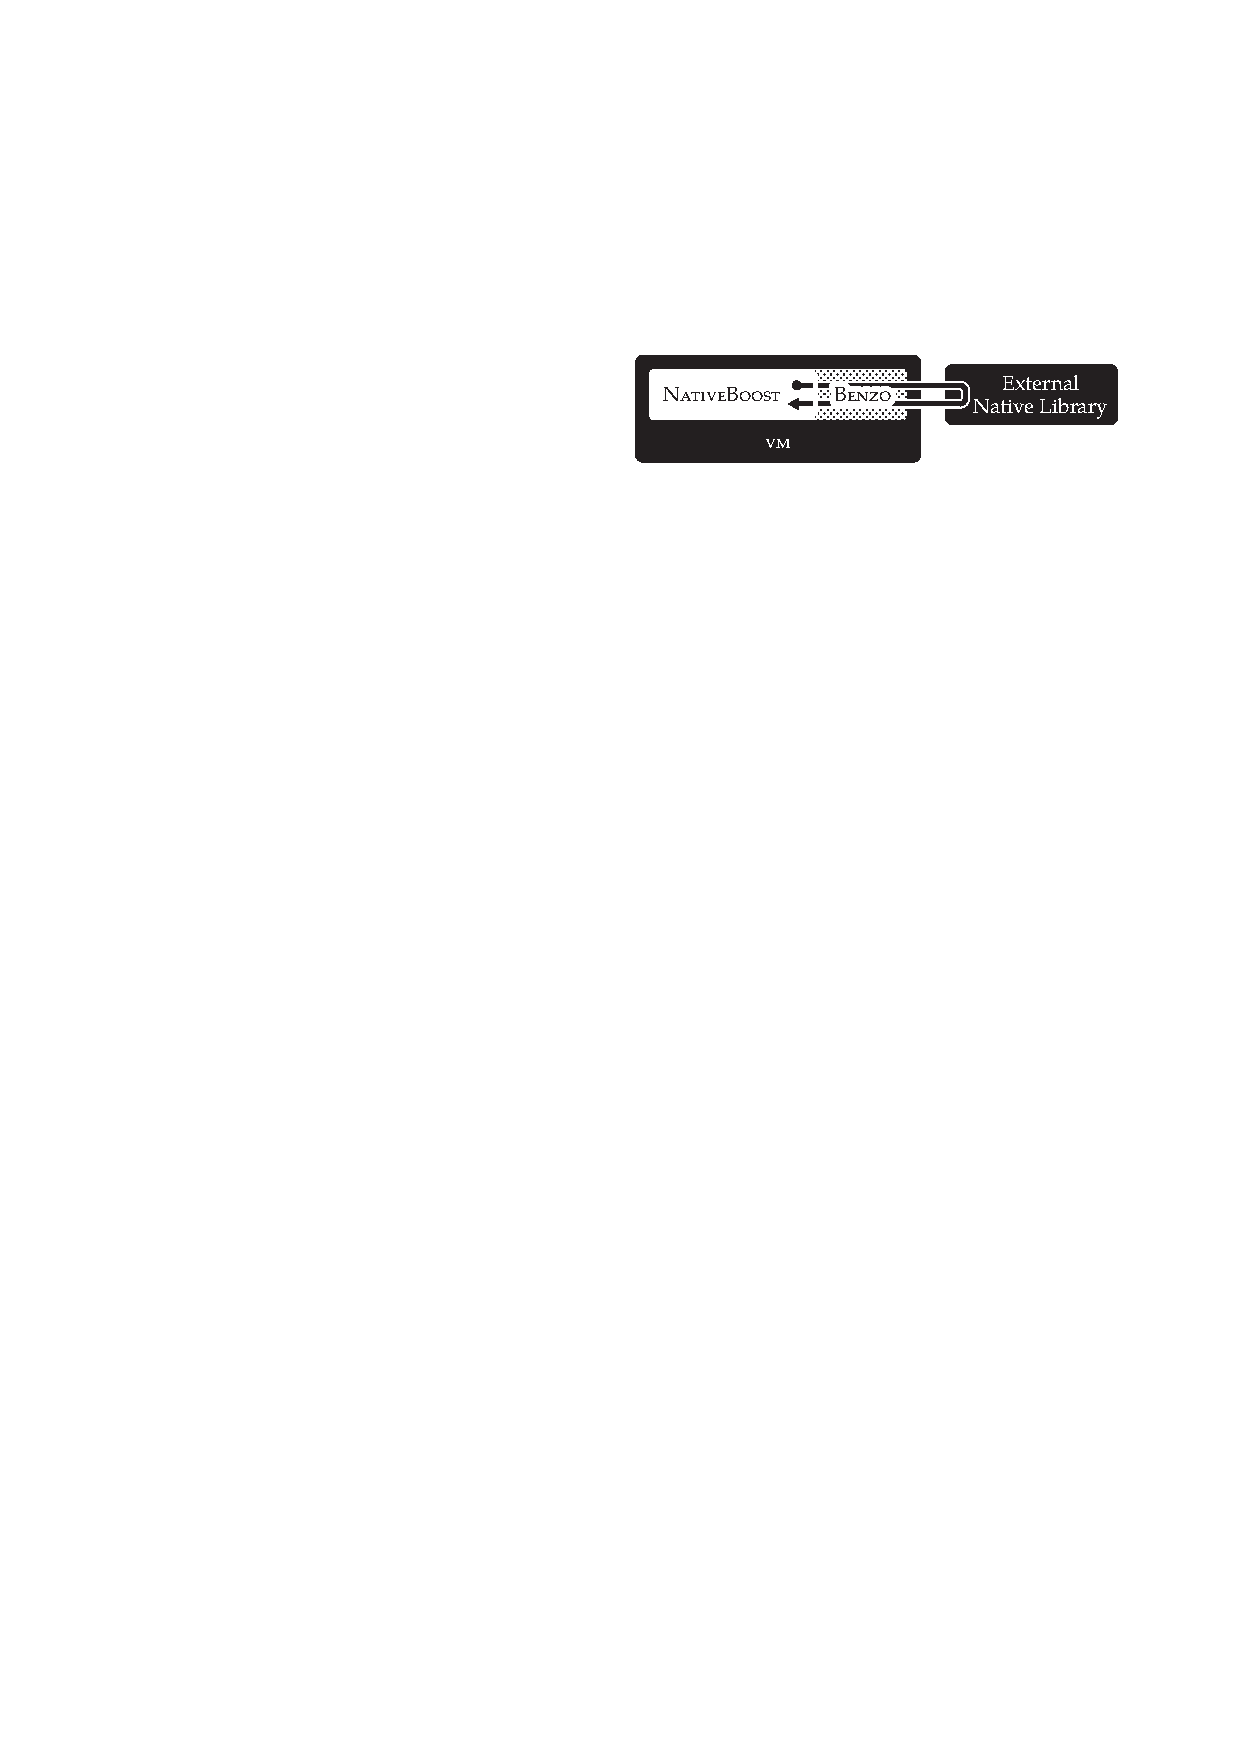
\includegraphics[scale=1.1]{nativeboost-overview}
	\caption[\NB Overview]{\NB generates generates native code at language-side with \B to perform an \FFI callout to an external function.}
	\figlabel{benzo-ffi-overview}
\end{figure}

\noindent \FFIs enable a programmer to call external functions without the need to implement additional \VM extensions.
\NB \cite{Brun13a} is a production-ready \FFI for \PH, developed on top of \B. 
For a detailed discussion of the implementation of \NB see \chapref{ffi}.
An \FFI implementation consists of two main parts: calling external functions and converting data between the two environments.
Typically a big percentage of these two parts are implemented at \VM-level with statically defined bindings.
Relying on \B's capability to dynamically generate and execute native code we developed a complete \FFI at language-side.
This way the \VM no longer requires to have a specific \FFI extension.

A very simple example to illustrate the functionality of \NB is to access the current environment variables with the \ttt{getenv} C function.
\ttt{getenv} takes a name as single argument and returns the value of that environment variable as a string:
%
\begin{stcode}{4}
getenv: name
    ^ NativeBoost call: 'String getenv(String name)'
\end{stcode}
%
In this example \NB automatically detects, using reflection, that the argument for the \PH method corresponds to the one of the low-level C function.
The most important aspect about this example is that it is written with standard \PH code, a property that extends to almost the complete implementation.
\NB, additionally to the native code activation, relies on two simple primitives provided by \B to retrieve addresses of external functions (\ttt{dlsym}) and to load external libraries (\ttt{dlopen}).

\NB generates the glue code to call external functions dynamically at run time.
It relies on \B's features presented in \secref{benzo-language-side} to generate and activate native code at runtime.
This gives \NB a significant advantage over static approaches: the generated native code is specific to the callout.
For instance in the \ttt{getenv} example, the marshalling code for converting from the internal \PH strings to C strings is written a small assembler routine.
In this specific context, the assembler code is faster than any language-side code.
Yet \NB is very flexible since all these conversion routines are defined at language-side. 
Each language-side library can define its own highly efficient conversion routines for types that are used in \FFI callouts, which is not directly possible to do with a \VM extension.


%----------------------------------------------------------------------------
\subsection{Reflective Primitives}
\seclabel{benzo-waterfall}
%----------------------------------------------------------------------------

\begin{figure}[h]
	\centering
	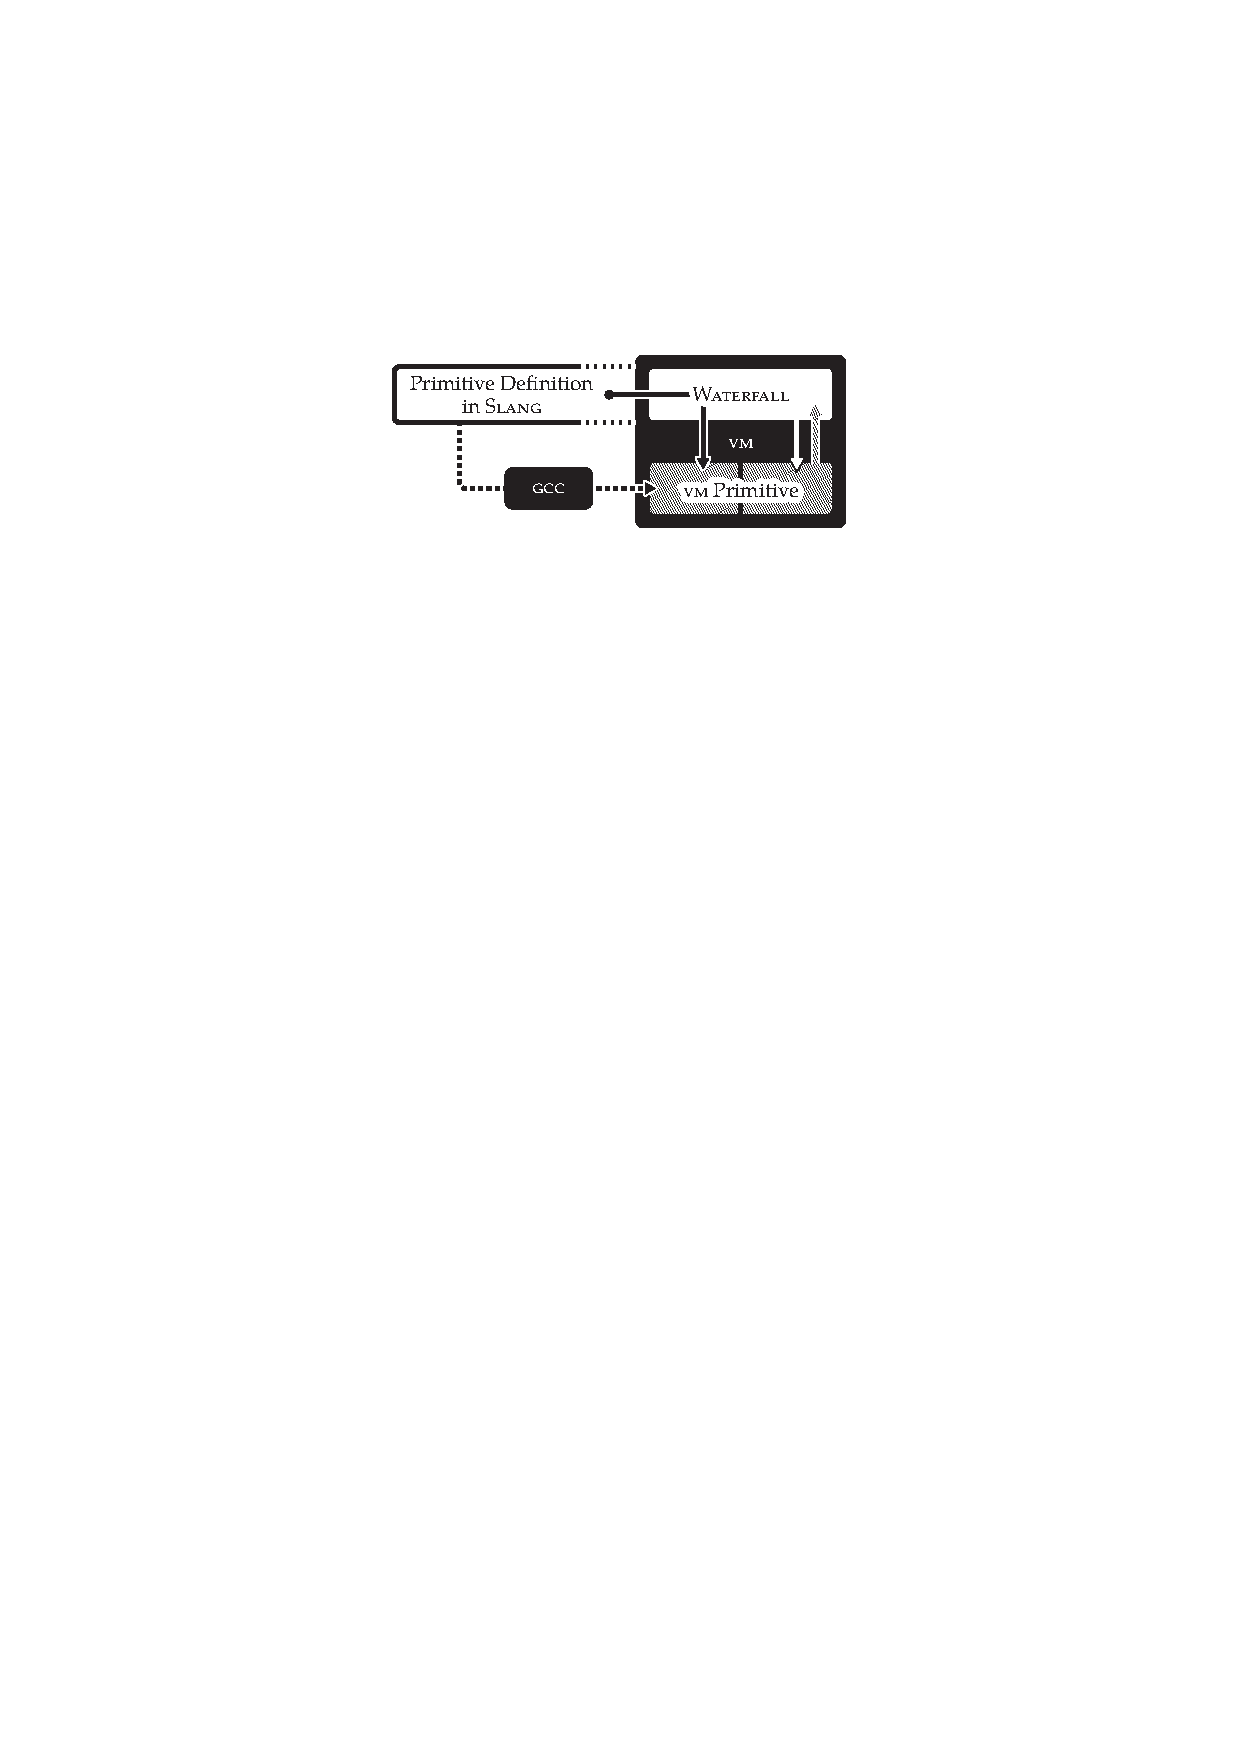
\includegraphics[scale=1.1]{waterfall-overview}
	\caption[\WF Overview]{\WF reuses the definitions of \VM primtives written in \Slang and compiles them dynamically. The same primitive definition is used for generating the static primitive at \VM compilation time.}
	\figlabel{benzo-waterfall-overview}
\end{figure}

\noindent The second \B-based application we present takes the concept of our \FFI solution further.
\NB allows us to call external functions by generating the callout code at language-side.
From an abstract point of view we replace language-side methods with native routines.
\NB does not directly synthesize new features but only makes external functionality available to the language itself.

As explained previously in \secref{benzo-vm-interaction} \B uses \PH's primitives to activate native code.
Since \PH is an open system we can extend this behavior to existing methods.
Instead of simply adding new methods which call native code we present \WF, a solution that modifies existing primitive methods and replaces them with \B-based native code.
Instead of manually generating the sources for the primitives we reuse existing code.
The \VM used for \PH is metacircular, the \VM sources are written in the same language, in our case in a simplified subset of \PH called \Slang.
Hence, the complete definition of the \VM including the primitives can be made accessible at language-side by loading the \VM sources.
\WF then takes the primitive definition written in \Slang and compiles it to native-code.

As \figref{benzo-waterfall-overview} illustrates, \WF extends the lifetime of the metacircular \VM definition to the actual language runtime.
By default the primitive definitions written in \Slang are only used to generate the \VM source in an intermediate step.
A C-compiler such as \GCC generates the final binary.
By doing so the high-level primitive definition are absorbed by the intermediate compiler infrastructure.
The final binary has no reflective capabilities anymore.
From within \PH we can only activate primitives but the abstract definition is no longer accessible.
Hence, we can not directly modify primitives directly without the original \VM sources loaded.

\WF provides a complete metacircular infrastructure for primitives.
We use \WF to modify primitives on the fly.
For instance it becomes possible to instrument the crucial \ttt{basicNew} primitive, something that is almost impossible to achieve with pure language-side reflection.
Since this primitive is used for object creation, each attempt to monitor this primitive is doomed.
If the monitoring code itself would create a new object, infinite recursion would be inevitable.
In \secref{val-waterfall} we explain in more detail the difficulty of such a task along with promising performance evaluations.



%----------------------------------------------------------------------------
\subsection{\NBJ \JIT Compiler}
\seclabel{benzo-nabujito}
%----------------------------------------------------------------------------
In this section we present \NBJ, a \B-based approach for a language-side \JIT compiler.
\NBJ goes even further than \WF using almost the same techniques.
However, instead of focusing on primitives, \NBJ generates native executable code for standard \PH methods.
Primitives tend to be more low-level, whereas \NBJ focuses on high-level \PH code. 

\begin{figure}[h]
	\centering
	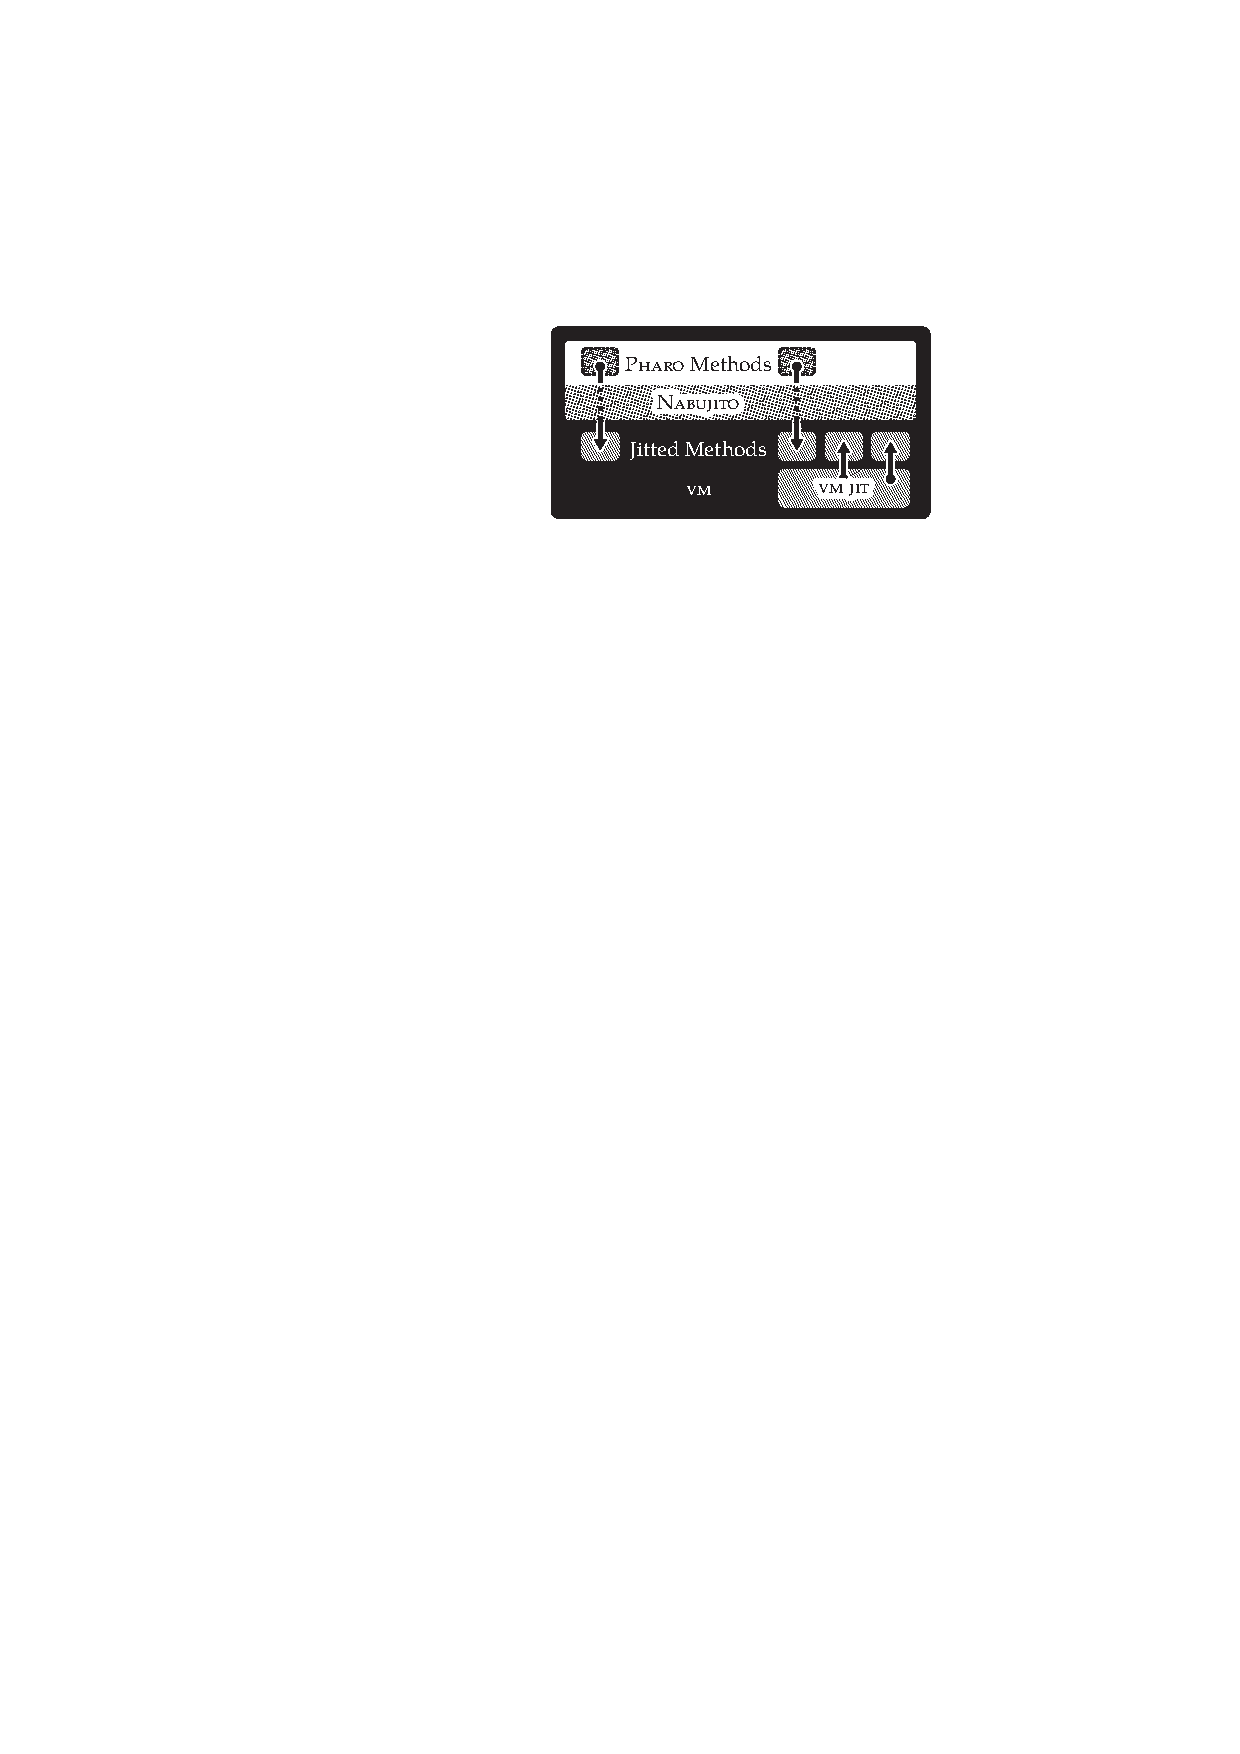
\includegraphics[scale=1.1]{nabujito-overview}
	\caption[\NBJ Overview]{\NBJ compiles standard \PH methods with the help of \B to the same format the \VM \JIT uses.}
	\figlabel{benzo-nabujito-overview}
\end{figure}

\noindent The \PH \VM (originally \urlfootnote{\textsc{Cog vm}}{http://www.mirandabanda.org/cog/}) already comes with a \JIT that translates bytecodes to native instructions.
It transforms \PH methods into slightly optimized native code at runtime.
The most complex logic of the \JIT infrastructure deals with the dynamic nature of the \PH environment.
Methods and classes can be changed at runtime and that has to be addressed by the \JIT infrastructure.
This implies that an efficient \JIT infrastructure needs substantial access to language-side structures; in our case classes, methods.
This information is readily accessible in \PH through the standard reflective \API.
However, at \VM-level this requires more effort, and thus imposes strong requirements on the design of classes and methods at language-side.
The \JIT infrastructure is a hybrid between \VM logic and language-side reflection.

The \JIT compiler, by which we refer in this context to the transformation of bytecodes to native code, represents a small part of the whole \JIT infrastructure.
There exists more important stages as an additional register allocation pass to reduce the number of stack operations \cite{Mira99a,Mira11a}.
The existing \JIT infrastructure is implemented in \Slang \cite[Ch.\ 5]{Blac09a} as the rest of the \VM.
We believe that a hard-coded static and low-level implementation is not optimal for several reasons:

\begin{itemize}
	\item Optimizing \PH code requires strong interactions with the dynamic environment.
	\item Accessing language-side properties from the \VM-side is hard.
	\item Changing the \JIT compiler requires changes at \VM-level.
	\item The \JIT reimplements primitives for optimization reasons resulting in code duplication.
\end{itemize}

\paragraph{Implementing \NBJ with \B.}
Motivated by the aforementioned implications of a \VM-level \JIT we conceived \NB a prototype \JIT compiler based on \B.
\NBJ is an experimental \JIT implementation which replaces the bytecode to native code translation of the existing \JIT infrastructure with a dynamic language-side implementation.
\NBJ is implemented as a visitor over the existing intermediate bytecode representation. 
Additionally we reimplemented vital native routines for the \JIT which are not directly exported by the \VM using \B. 
\NBJ relies on the following \VM-level infrastructure to manage and run native code for any \PH method:

\begin{itemize}[noitemsep]
	\item Fixed native code memory segments.
	\item Routines for switching contexts.
	\item Native stack management.
\end{itemize}

\paragraph{Dynamic Code Generation.}
For standard methods \Nabujito takes the bytecodes and transforms them to native code.
It also applies optimizations such as creating low-level branches for \PH level branching operations like \ttt{ifTrue:}.
Optimizations for additional methods are all implemented flexibly at language-side.
Wherever possible, we reimplement the same behavior as the existing native \JIT compiler.
Eventually the native code is ready and \B attaches it to the existing compiled method.
When the language-side jitted code is activated \B ensures that we do not have to leave the \JIT execution mode, and thus we can call methods at the same speed as the existing \JIT.
\secref{val-nabujito} gives a more detailed insight of the design and performance of \NBJ.


%============================================================================
\section{Performance}
\seclabel{benzo-issues-performance}
%============================================================================
\todo{Shorten this section and put forward pointers to the real validation chapters yet to come (copied contents, feel free to distroy...)}
In this section we discuss the general performance characteristics of \B for the three example applications outlined in the previous section.
A more detailed validation is presented later in \secref{ffi-performance} (\FFI), \secref{val-waterfall-performance} (\WF) and \secref{val-nabujito-performance} respectively.

\paragraph{One-time Code Generation Overhead.} 
\B allows the generation of specific and thus efficient native code.
In \secref{benzo-benzo} we explained how \B causes only a one-time overhead for native code generation. 
Thereafter it is cached for later activations.
The three use case presented in \secref{benzo-usecase} heavily benefit from this fact.
Even though the code generation at language-side is generally slower than a C-level implementation, the overhead can mostly be neglected.
Even better, for instance the \B-based \FFI implementation presented in \secref{benzo-ffi} outperforms a \VM-level \FFI-plugin due to a more flexible language-side implementation. 
These results are shown in the following \tabref{benzo-ffi-performance-simple}.

% ---------------------------------------------------------------------------
\subsection{\B-based \FFI}
\seclabel{benzo-nb-performance}
% ---------------------------------------------------------------------------

The first mini performance evaluation we present is for \NB the \B-based \FFI.
Compared to a static plugin-based \FFI implementation \NB has only a one-time startup overhead with its numbers shown in \secref{benzo-issues-performance}.
Generating the native code at language-side is substantially slower than directly setting up all the conversions and calling the external functions from C code. 
In some cases the penalty for some compilation effort on \NB is as high as a factor of 100 compared to classic approaches.
Under the assumption that the method is called several times this overhead may be considered negligible.
An in-depth evaluation of \NB comparing against other solutions is presented later in \chapref{ffi}.
The following table contains a performance comparison of three different \FFI implementations for \PH that represents the typical showcase.

\begin{table}[!ht]
    \centering
    \begin{tabular}{rSS}
                   					& {Call Time [ms]} & {Relative Time} \\\midrule
        \NB         				& 10.53(35)        &        1.0 \\
        \Alien, language-side \FFI  & 31.09(94)        & \approx3.0 \\
        C-\FFI, plugin-based \FFI   &  9.55(64)        & \approx1.9
    \end{tabular}
    \caption[Basic \B-based \FFI Performance]{Different \FFI implementations in \PH evaluating \ttt{abs(int)}. \Alien does marshalling at language-side while \FFI does everything in \VM plugin written in C.}
    \tablabel{benzo-ffi-performance-simple}
\end{table}

\tabref{benzo-ffi-performance-simple} measures the accumulative time of 100'000 \FFI calls.
Included in these numbers is at least one additional \PH message send to activate the \NB method containing the actual call to the C function.
\NB outperforms the existing language-side \FFI (\Alien) and the implementation (C-\FFI).

The existing language-side \FFI has a generic plugin to call C-functions and performs type-conversions at language-side.
However, converting \PH objects from and into low-level data is comparably expensive.
In \NB this happens directly in custom generated native code and is thus significantly faster.

The plugin-based \FFI is also slower than \NB since it still has generic conversion function for \PH objects, albeit written in C and thus faster than in \Alien.
However, \NB custom tailored \ASM code is still faster than the hard-coded C counterpart.

This simple \FFI evaluation already highlights the core benefit of \B to generate very customized native code when needed.
Yet we have to emphasize that \NB is based on the \B infrastructure whereas the other solutions require both a \VM plugin whose sole purpose is to enable the \FFI functionality.
Furthermore \NB benefits from the the \JIT interaction described in \secref{benzo-jit-interaction}.
This optimization is especially an important optimization factor when calling out small helper routines where the context switch from jitted mode is no longer negligible.

% ---------------------------------------------------------------------------
\subsection{\B-based Dynamic Primitives}
\seclabel{benzo-wf-performance}
% ---------------------------------------------------------------------------

As the second mini performance evaluation of \B we present a simple use case of dynamically implementing a primitive with \WF.
For comparing performance we implement a very simple integer operation primitive (\ttt{$>$}) using three different approaches.
The first approach is the implementation with \WF.
The second is to run the language-side implementation that is triggered whenever the standard primitive failed.
Finally the fast standard primitive provided by the \VM.
We run the three approaches by measuring the cumulative time over one million primitive activations averaged over 100 runs.
The absolute numbers are less important than the relative factor between them.
We present the results of this experiment in \tabref{benzo-waterfall-performance}.
%
\begin{table}[!ht]
    \centering
    \begin{tabular}{rSS}
		Primitive Type  & {Running Time [ms]} & {Relative Time} \\\midrule
		\VM			    &   6.40(14)          &         1.0 \\
		\WF             &  22.80(17)          & \approx 3.6 \\
        Reflective	    & 195.00(16)          & \approx30.0
    \end{tabular}
    \caption[Basic \B-based Dynamic Primitive Performance]{Comparing running time of different implementations of integer arithmetic primitive.}
    \tablabel{benzo-waterfall-performance}
\end{table}
%
\WF clearly outperforms a purely reflective solution.
As explained in \secref{benzo-waterfall}, replacing a crucial primitive with simple language-side is not straight forward.
If the replacement code triggers the very same primitive again we are trapped in so called meta-recursion.
To avoid this, the \PH code for the replacement of \ttt{$>$} checks that the current activation of the primitive is not recursive.
This comes at a substantial cost and is the main overhead factor.

\WF is a factor $3.6$ slower than the standard implementation.
First we have to state that \WF uses a very simplistic compilation strategy with many optimizations opportunities left out.
Second, the optimized \VM primitive is also reimplemented in the \JIT to avoid the overhead of switching execution context (see \secref{benzo-vm-interaction}).

This results thus makes a whole new set of runtime extensions feasible that were previously limited by their strong performance penalty.
Furthermore the performance penalty over a completely optimized \VM solution that has extreme optimization techniques, such as inlining and register allocation, is less than a factor of $4$.
A more detailed analysis of \WF is available later in \secref{val-waterfall-performance}.

% ---------------------------------------------------------------------------
\subsection{\B-based \JIT compiler}
\seclabel{benzo-nabujito-performance}
% ---------------------------------------------------------------------------

The performance evaluation for our \B-based \JIT compiler is focused on the language-side code-generation part a more detailed discussion is given in \secref{val-nabujito-performance}.

\NBJ essentially generates the same native code as the \VM-level \JIT, hence there is no performance difference at evaluation time.
However, \NBJ is clearly slower during the warm-up phase.
Compilation of the native instructions will take considerably more time compared to the \VM-level implementation of the same bytecode to assembler transformation.
The cost of transforming the bytecodes to native code at \VM-level can be measured in native instructions, whereas the unit at language-side is bytecodes.
However, we point out again, that this is a one-time overhead.
From the in-production experience of \NB, the \B-based \FFI (see \secref{benzo-nb-performance}), we know that these costs amortized, especially for long-term applications.
Instead of focusing on the final performance of the generated code, we present the compilation time compared to the normal \PH bytecode compiler, which also resides at language-side.

\begin{table}[!ht]
    \centering
    \begin{tabular}{rS}
                      & {Compilation Time [ms]} \\\midrule
        \PH Compiler  & 71(1) \\
        \NBJ          & 73(1)
    \end{tabular}
    \caption[Basic \B-based \JIT Performance]{Compilation efforts of the standard \PH compiler in \PH and \NBJ for the a simple method returning the constant \ttt{nil}.}
    \tablabel{benzo-nabujito-performance-small}
\end{table}

In \tabref{benzo-nabujito-performance-small} we compare the compilation speed of the standard \PH compiler and \NBJ.
We measure the accumulated time spent to compile the method 1000 times.
The average and deviation are taken over 100 runs. 
The \PH compiler takes source code as input and outputs \PH bytecodes.
\NBJ takes bytecodes as input and outputs native code.

We see that in the simple case displayed in \tabref{benzo-nabujito-performance-small} \NBJ's compilation speed lies within the same range as the standard \PH compiler.
We expect that in the future we apply more low-level optimizations and thus increase the compilation time of \NBJ.
However, we have shown in the performance evaluation for \NB, the \B-based \FFI, in \secref{benzo-nb-performance} that even a rather high one-time overhead is quickly amortized.
Furthermore with \PH's image approach the generated native code is persistent over several sessions.
A subsequent restart of the same runtime will not cause the \JIT to nativize the same methods it did during the last launch.
Hence our approach is even valid for short-timed script-like applications as most of the methods will already be available in optimized native code from a previous run.


% ===========================================================================
\section{Related Work}
\seclabel{benzo-related}
% ===========================================================================
In the context of \B we have to respect a variety of related work spawning different abstraction levels.
On a more abstract scale \B allows for a new way of extending the complete language runtime, hence we classify the related work according the following categories show in \figref{benzo-extensionComparison}: general language-side extensions, extensions using reflection, \VM-level extensions, and hybrid approaches.

We present now an overview of the approaches used to extend a language runtime and expose their limits.
High-level languages are in general sustained by a \VM and a vast set of libraries written in the language itself. 
Extending or improving the existing language runtimes is a difficult task.
In most cases the \VM is considered as a black box.
Additionally the \VM is written in a completely different language using another abstraction level than the one it supports.
Typically high-level language \VMs are written in C or C++.
To address extensions in this context there exist some known approaches:

\begin{description}[noitemsep]
	\item[Language-side Library] based on implementing a new or existing library. 
	\item[Reflective Extension] relying on reflective features of the language. 
	\item[\VM Extension] by writing plugins or changing the core of the \VM.
	\item[Hybrid Extension] by accessing external libraries using \FFI.  
\end{description}
%
The relation between the side concerning the abstraction and implementation levels (\VM vs. language) of these extensions is illustrated in \figref{benzo-extensionComparison}.

\begin{figure}[h]
	\centering
	\begin{subfigure}[t]{0.45\textwidth}
		\centering
		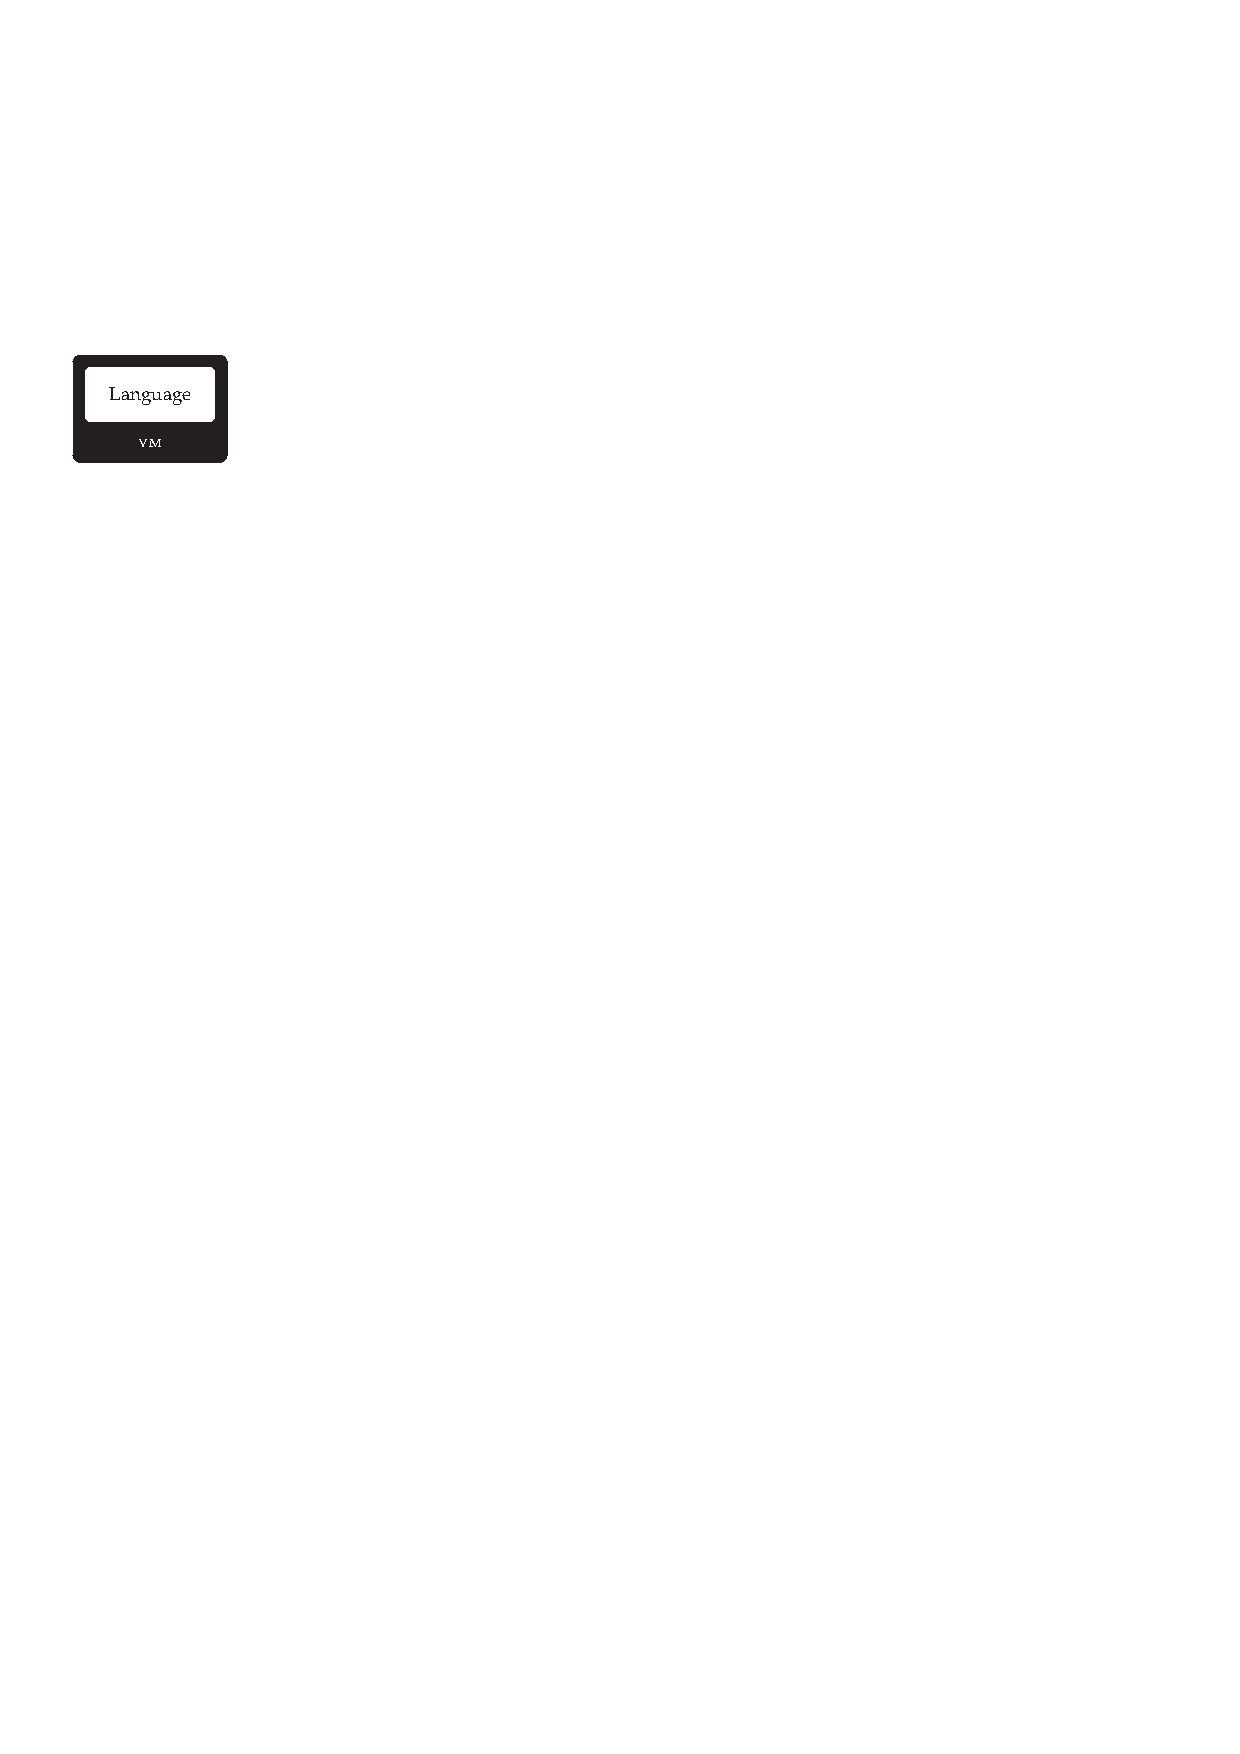
\includegraphics[scale=1.1]{extension-language}
		\caption{Language running on a standard \VM.}
	\end{subfigure}\hspace{0.09\textwidth}
	\begin{subfigure}[t]{0.45\textwidth}
		\centering
		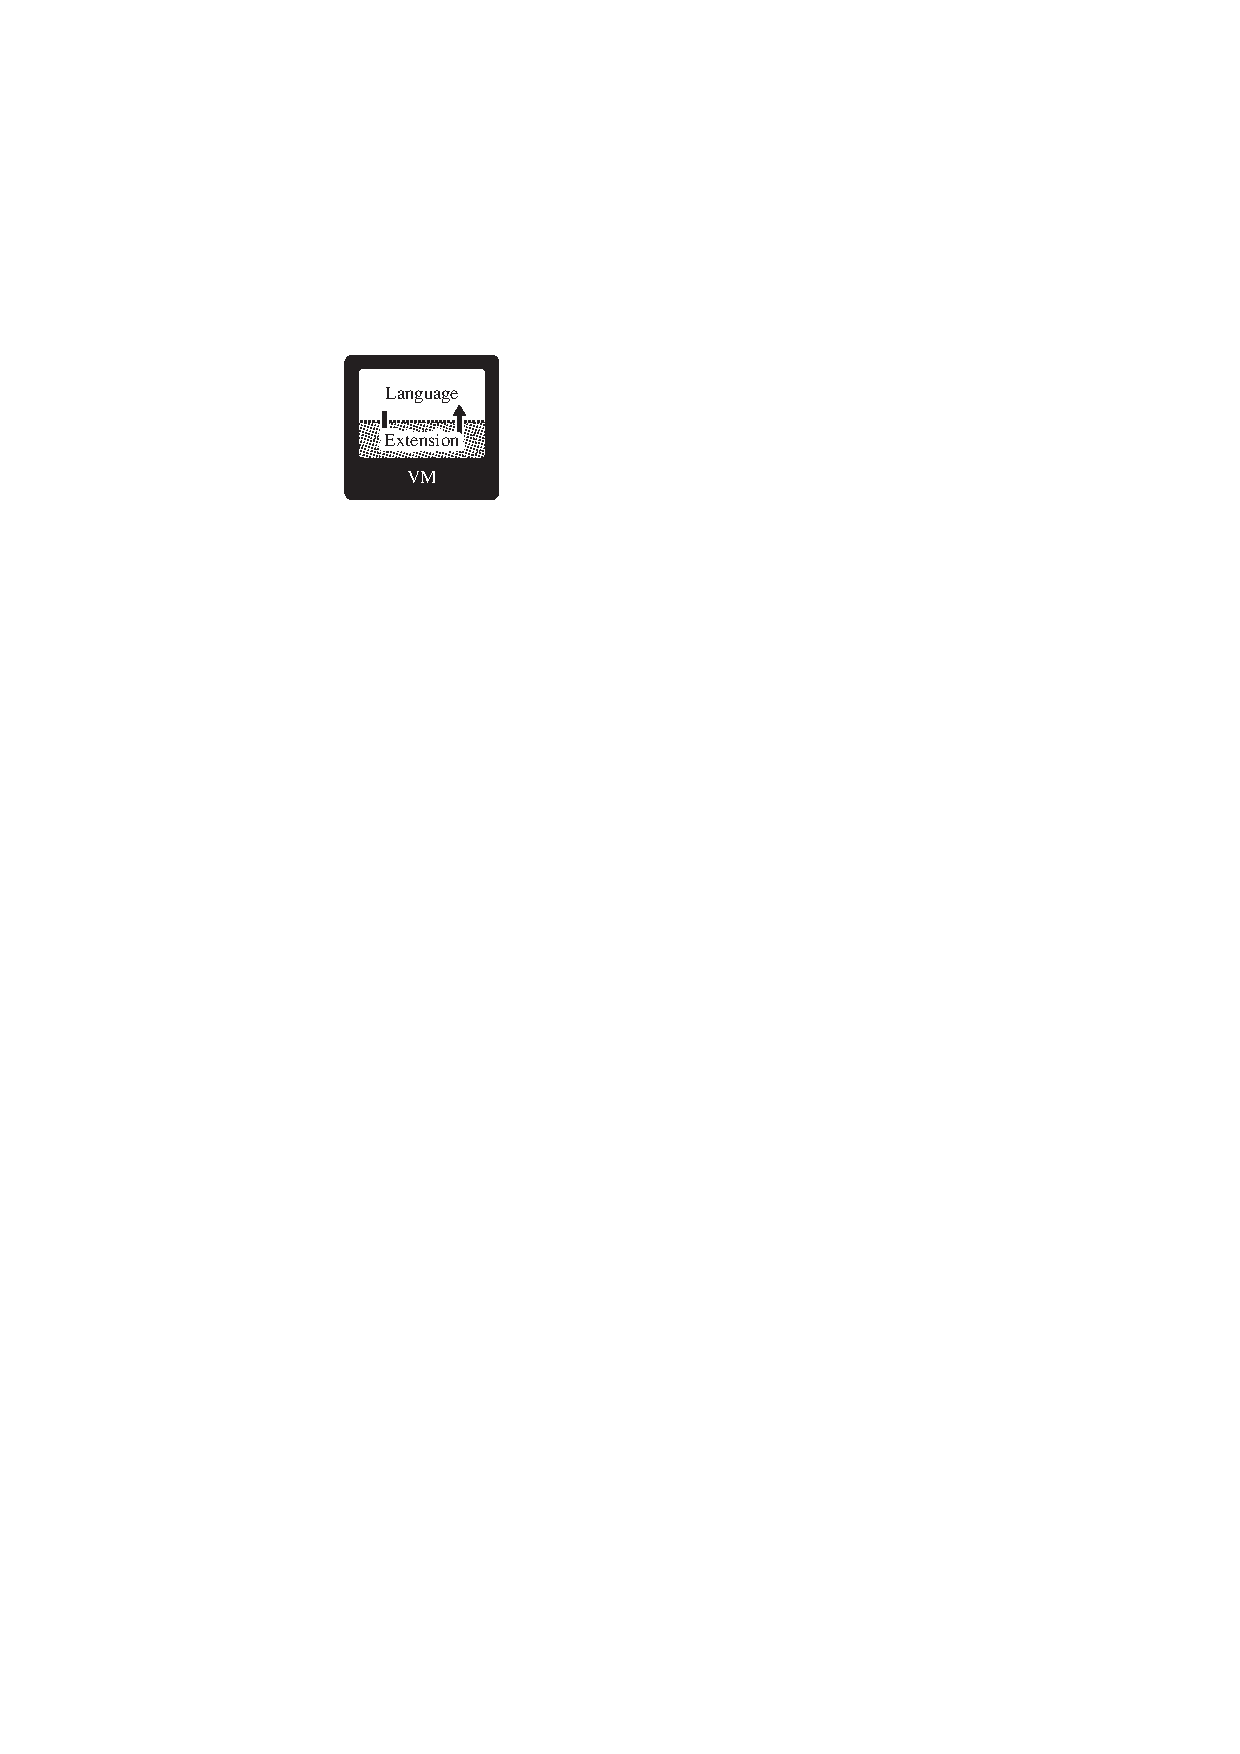
\includegraphics[scale=1.1]{extension-language-library}
		\caption{Language-side implementation of an extension.}
	\end{subfigure} \\
	\vspace{\baselineskip}
	\begin{subfigure}[b]{0.45\textwidth}
		\centering
		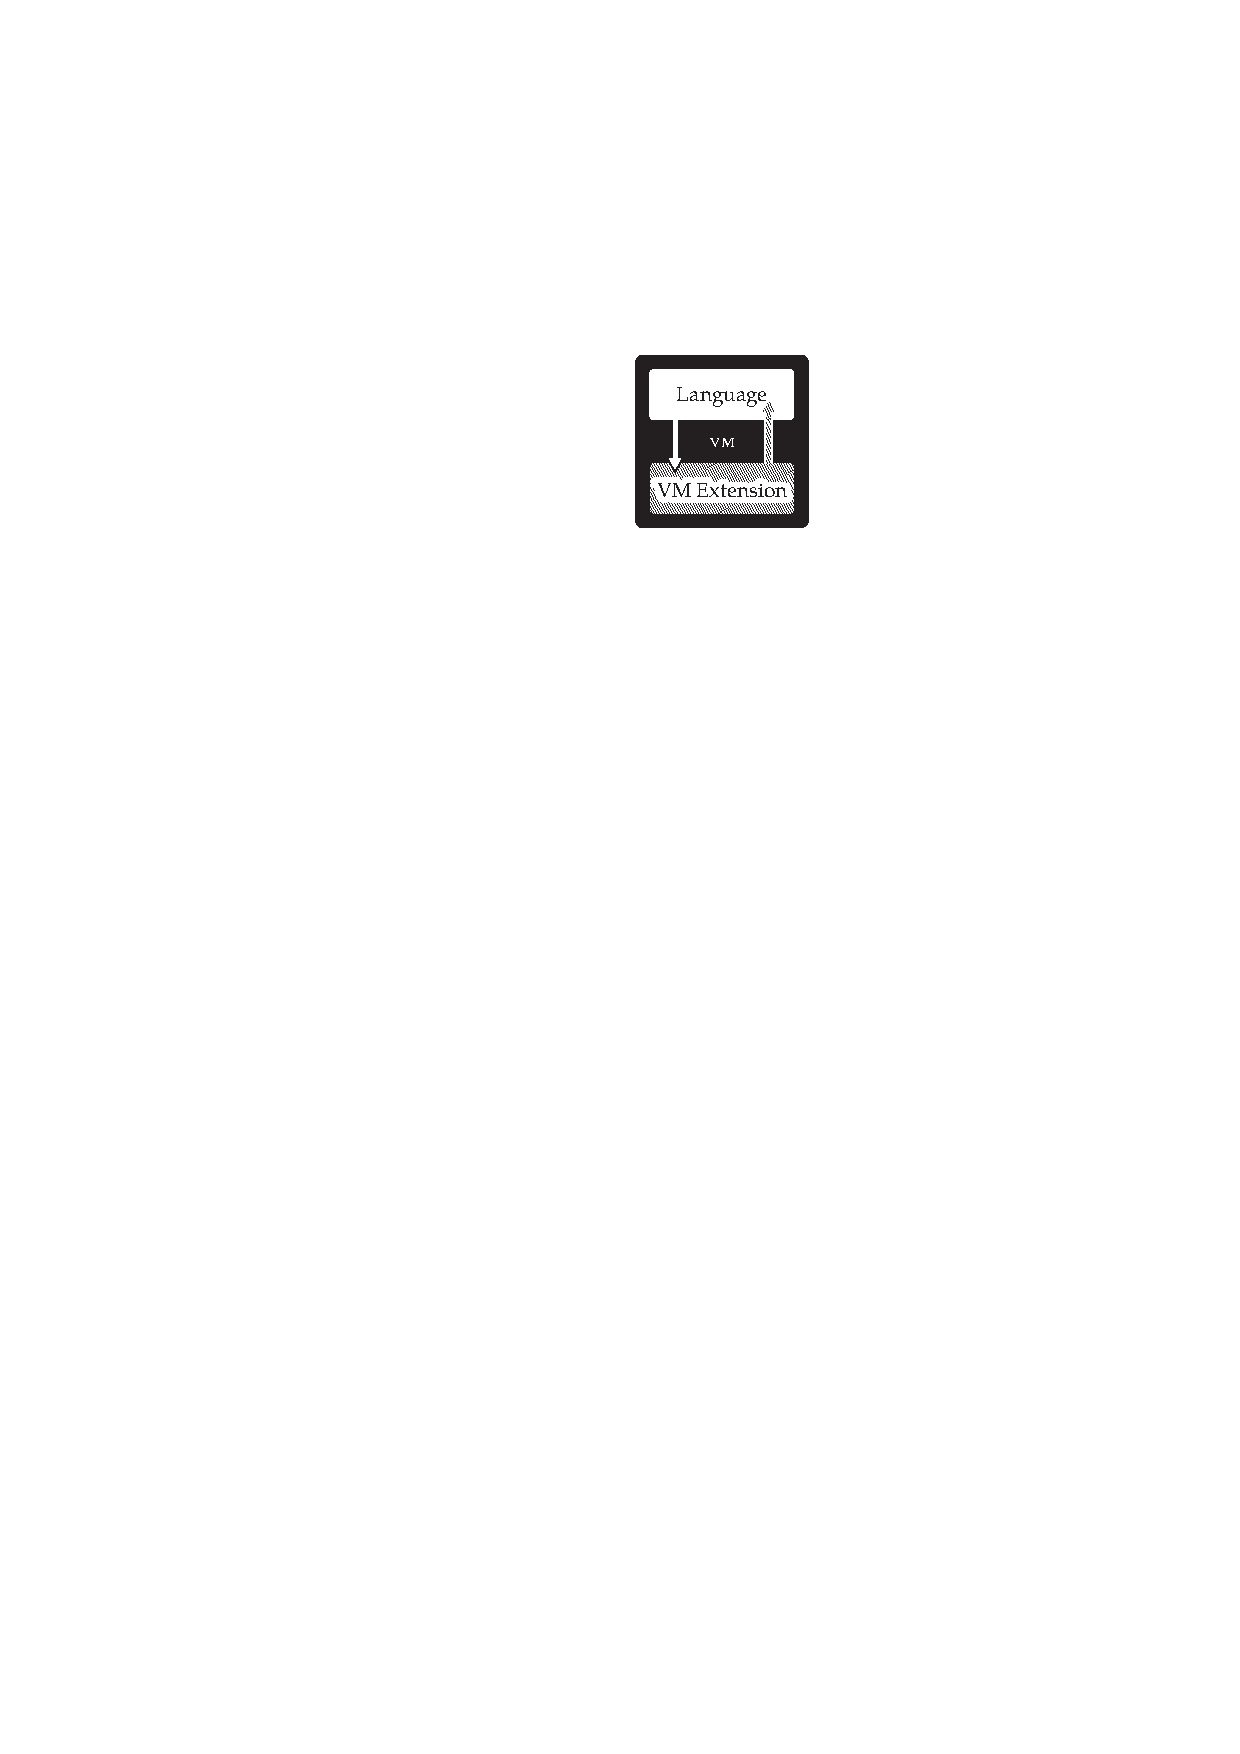
\includegraphics[scale=1.1]{extension-vm}
		\caption{Language using features from a \VM extension.}
	\end{subfigure}\hspace{0.09\textwidth}
	\begin{subfigure}[b]{0.45\textwidth}
		\centering
		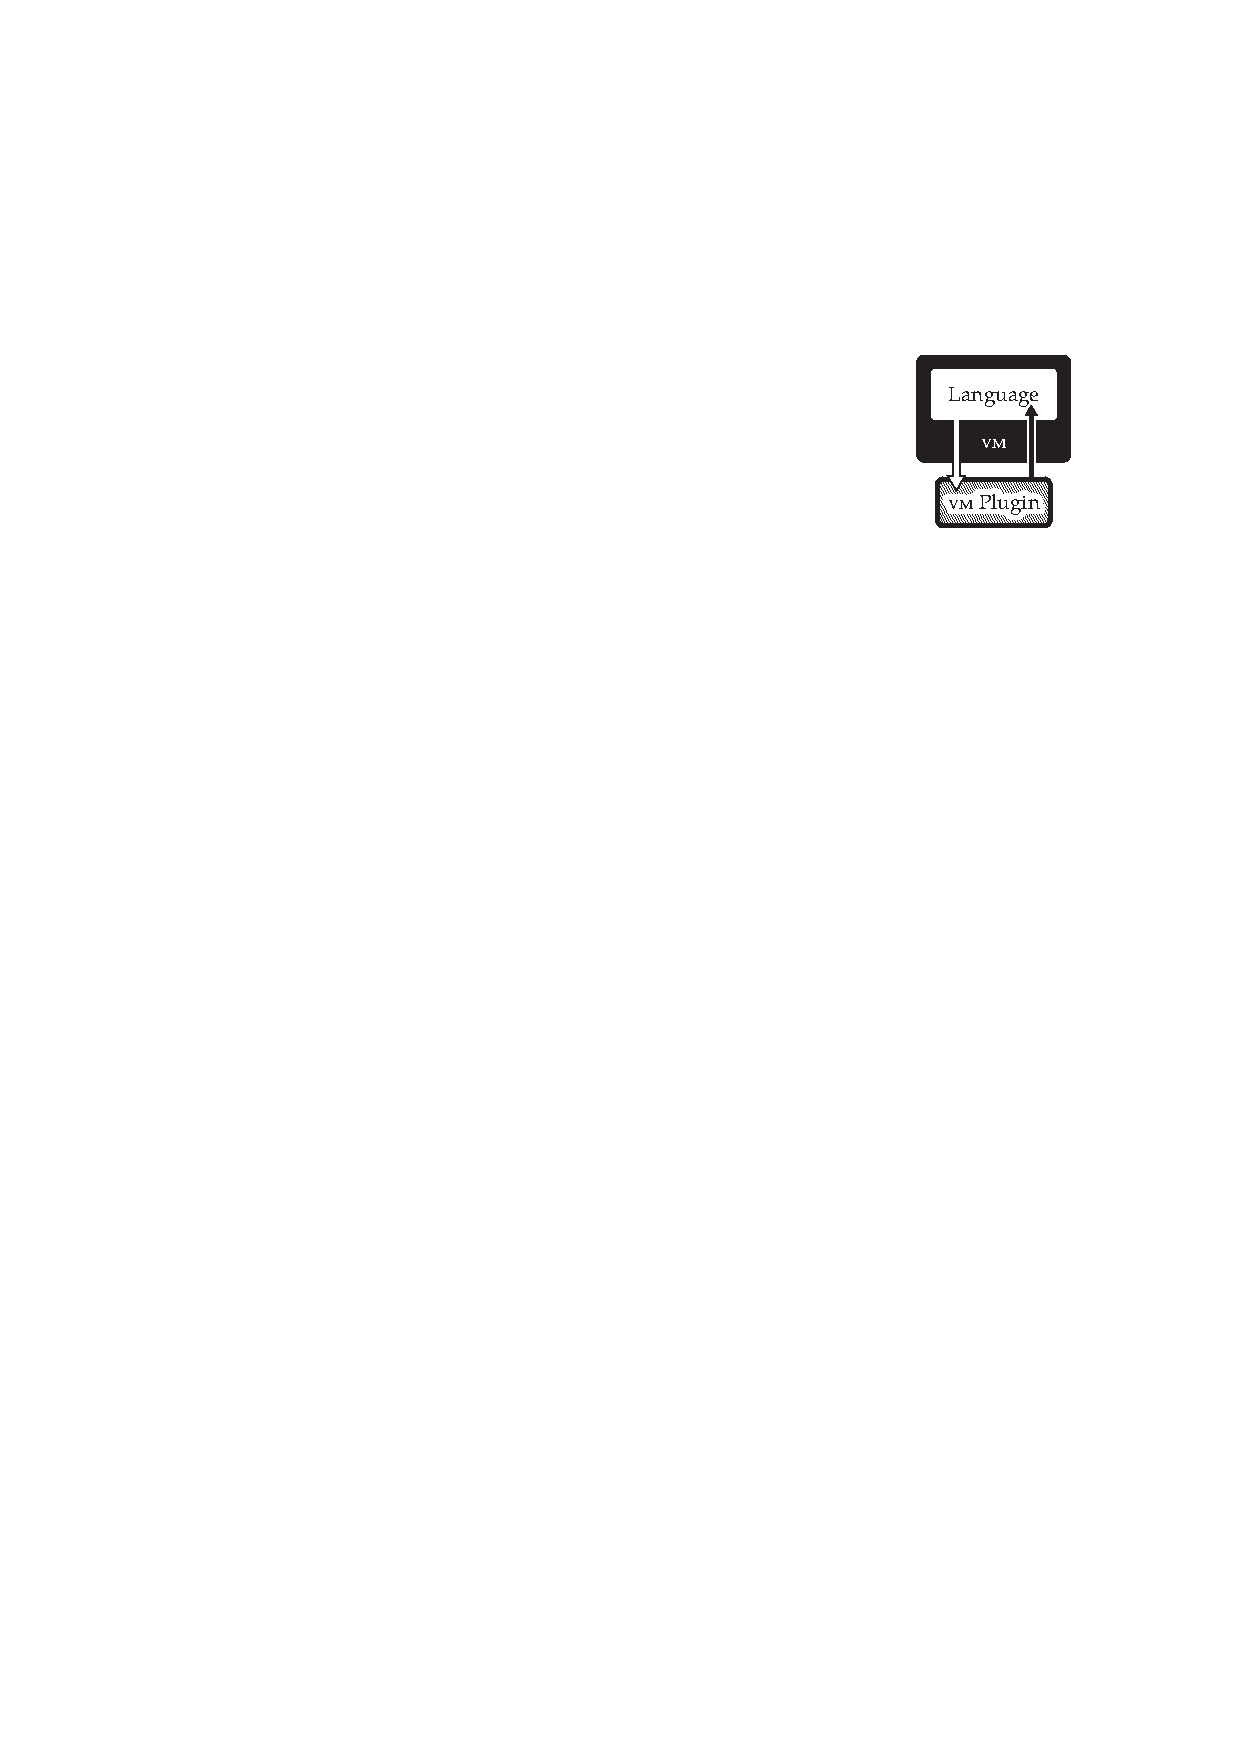
\includegraphics[scale=1.1]{extension-plugin}
		\caption{Language using features from a separate \VM plugin.}
	\end{subfigure}
	
	\caption[Language Extension Mechanisms]{Comparison of different extension mechanisms}
	\figlabel{benzo-extensionComparison}
\end{figure}

%----------------------------------------------------------------------------
\subsection{Language-side Library}
%----------------------------------------------------------------------------

The most straight forward solution for extending a language is to write libraries within the language itself. 
This option provides the advantage that the aggregate behavior is accessible and evolvable for any language developer.
However, language-side libraries are constrained by the underlying managed language runtime.
The \VM separates the language from the low-level internal details.
As a consequence language-side libraries are not feasible for all feature requirements.
For instance the previously mentioned example of instrumenting the language runtime is not possible as a standard language-side extension without a considerable performance loss.
So, even though we prefer extensions and optimizations at language-side, there are certain limitations of a managed language runtime that can not be circumvented.
If all language-side optimization opportunities have been exhausted it is exposing the need to resort to lower level approaches.

\begin{quote}
Language-side libraries are constrained to the capabilities of the underlying \VM and thus not general enough. 
Additionally not all performance bottlenecks can be addressed at language-side.
\end{quote}

%----------------------------------------------------------------------------
\subsection{Language-side Reflective Extensions}
%----------------------------------------------------------------------------

This is a subcase of the previous approach but in the context of reflective environments that expose particular characteristics.
For instance, Meta Object Protocols (\MOP) \cite{Kicz91a} based on reflection \cite{Maes87a} are used to define certain control points in the system to change the language.
By composing meta objects it is possible to even modify the semantics of the language. 
Several languages such as \PH, \ST, \urlfootnote{\Python}{http://python.org/}, \urlfootnote{Ruby}{http://www.ruby-lang.org/}, and others provide reflective capabilities with different depths \cite{Ande98a,Van10a}.
However, most modern programming languages only have very limited support for intercession.
Hence the possibilities for dynamically changing language semantics or features are limited. 
Furthermore reflective capabilities are hard to implement efficiently.
Reflection imposes substantial performance penalties on most computations by postponing bindings \cite{Male96a}. 
Nevertheless, there are exceptions for a subset of reflective behavior which are implemented efficiently using a high-level MOP \cite{Vran12a}.
Though these approaches remain as a few exceptions.
In the typical low-level \VM it is difficult to gain reflective access to language-side objects.
Similar to the previous case, our goal is to extend language features in a general way and it was shown that this is only partially possible by reflective extensions. 

\begin{quote}
Reflective capabilities are not enough for general extensions. Even when suitable, they usually pose a significant performance overhead up to the point where they become unfeasible.
\end{quote}

%----------------------------------------------------------------------------
\subsection{\VM Extensions.}
\seclabel{benzo-vm-extensions}
%----------------------------------------------------------------------------

Another approach is to attach plugins to the \VM.
Plugins are direct bindings to external libraries described at \VM-side or libraries linked to the \VM executable \cite[Ch.\ 5]{Blac09a}. 
They provide a performance boost in comparison to pure language-side solutions.
Using highly optimized native libraries it is straightforward to outperform code written at language-side.
However, plugins are commonly written in the same language as the \VM, at a low abstraction level.
Few exceptions are self-hosted languages \cite{Unga05a,Wimm13a,Rigo06a}.
To support a fluent development process, \VMs should come with an infrastructure for building extensions at same abstraction level than the language.
Instead they tend to be very complex and to have sluggish building processes. For example, only a few \VMs have high-level debugging facilities \cite{Inga97a,Unga05a,Wimm13a}.
Also from a \VM maintenance point of view, extensions have to be avoided if possible and should only be used for critical performance issues that can not be properly addressed at language-side.
An example of how the complexity of the \VM can affect development efforts is the core of the \Self \VM \cite{Unga07a}.
After reduced development resources parts of the complex but efficient compiler infrastructure had to be abandoned in favor of a more maintainable code-base.

\todo{properly integrate}
High-level low-level programming \cite{Fram09a} encourage to use high-level languages for system programming.
Frampton et al. present a low-level framework packaged as \textsc{org.vmmagic}, which is used as system interface for Jikes, an experimental \Java \VM.
Additionally their framework is successfully used in \textsc{mmtk} \cite{Blac04a} which is used independently in several other projects.
The \textsc{org.vmmagic} package is much more elaborate than \B but it is tailored towards \Java with static types.
Methods have to be annotated to use low-level functionality.
Additionally the strong separation between low-level code and language-side application does not allow for reflective extensions of the language runtime.
Finally, they do not support the execution nor generation of custom assembly code in the fly.

Other related approaches are \VM generation frameworks in general.
They try to abstract away the complexity of the \VM and use high-level languages as compiler infrastructure.
A very successful research project is \urlfootnote{\textsc{Jikes} Research \VM}{http://jikesrvm.org/} (former \textsc{Jalapeño})~\cite{Alpe99a}.
It uses \Java to metacircularly define a \Java environment which then generates the final \VM.

A similar framework is \urlfootnote{\PyPy}{http://pypy.org/} \cite{Rigo06a} a \VM framework including an efficient \JIT. 
\PyPy uses a restricted subset of the  \textsc{Python} language named \textsc{RPython} which is then translated to various low-level backends such as C or \textsc{llvm} code.
There exist several different high-level language \VM implementations on top of \PyPy such as \ST \cite{Bolz08a} or \textsc{Prolog}.
However, its main focus lies on an efficient \JIT generator mainly for a \Python interpreter, and not on a direct, language-side assembler interface.


\begin{quote}
VM extensions provide good performance at the cost of maintainability. 
Moreover this approach implies resorting to pure low-level development where tools and abstraction advantages from high-level languages are restricted.
\end{quote}

%----------------------------------------------------------------------------
\subsection{Hybrid Extensions}
%----------------------------------------------------------------------------
\todo{ensure that the \FFI related work is not that much}

The last approach is to reuse an existing library usually implemented in a foreign language.
The languages interact through a well-defined Foreign Function Interface (\FFI).
\FFI-based extensions are a hybrid approach between pure language-side extensions and \VM-side ones.
Interaction with native libraries is supported by a dedicated \VM functionality for calling external functions.
This allows for a smooth interaction of external code and language-side code.
\FFI-based extensions share the benefits of a maintainable and efficient language-side library with modest implementation efforts.
However, \FFI is only a bridge or interface for allowing the interaction of different languages. 
It is not possible to directly synthesize new native features from language-side.
For this purpose we have to interact with a custom-made native library.
From an extension point of view this is close to the \VM extensions discussed previously.

Additionally to the interface limitations, there exists a performance overhead in \FFI for making the interaction between different languages possible. 
This is due to marshalling arguments and types between both languages \cite{Fish00a,Repp06b}.


Other high-level languages such as \Lua leverage \FFI performance by using a close interaction with the \JIT.
\textsc{Luaffi}\footnote{\url{https://github.com/jmckaskill/luaffi/}} for instance is an efficient \Lua implementation that inlines \FFI calls directly into the \JIT compiled code.
Similar to \B this allows to minimize the constant overhead by generating custom-made native code.
\Luajit is mainly written in C which has clearly different semantics than \Lua itself.
Compared to our approach the efficient \VM implementation suffers from the shortcomings described in \secref{benzo-vm-extensions}. 

Kell and Irwin \cite{Kell11a} take a different look at interacting with external libraries.
They advocate a \Python \VM that allows for dynamically shared objects with external libraries.
It uses the low-level \textsc{Dwarf} debugging information present in the external libraries to gather enough metadata to automatically generate \FFIs.
However, they do not focus on the reflective interaction with low-level code and the resulting benefits. 

\textsc{Quicktalk} \cite{Ball86a} follows a similar approach as the dynamic primitives in \WF.
However, Ballard et al. focus mostly on the development of a complex compiler for a new \ST dialect.
Using type annotations \textsc{Quicktalk} allows for statically typing methods.
By inlining methods and eliminating the bytecode dispatch overhead by generating native code \textsc{Quicktalk} outperforms interpreted bytecode methods.
Compared to \WF \textsc{Quicktalk} does not allow to leave the language-side environment and interact closely with the \VM.
Hence it is not possible to use \textsc{Quicktalk} to modify essential primitives.

A notable exception to the metacircular \VMs mentioned earlier is the \Self implementation \textsc{Klein} \cite{Unga05a}.
Unlike typical other metacircular approaches it does not strictly separate compile-time and runtime.
The reified \VM concepts are available at runtime, which is a result from implementing the typical \VM pieces at language-side.
Compared to our approach, \textsc{Klein}'s bridging efforts are much more complete.
However, \textsc{Klein} is built on a completely new \VM infrastructure, whereas \B requires only few changes to achieve its functionality.

\begin{quote}
Hybrid extension are the most promising.
They allow for a seamless interaction from high-level language-side to low-level functionality.
However, most existing solutions target only specific use cases and can not be reused for other applications.
\end{quote}


% ===========================================================================
\section{Problems of Benzo}
\seclabel{benzo-problems}
% ===========================================================================
\todo{most problems are related to the missing debugging facilities}


% -----------------------------------------------------------------------------
\subsection{Robustness}
% -----------------------------------------------------------------------------
\todo{show a problematic piece of code} \\
\todo{sketch an outline for a safe benzo test by forking the main process} \\
\todo{image + code example} \\
\todo{possible emulation of the code to highlight very common bugs?}


% -----------------------------------------------------------------------------
\subsection{Low-level Debugging}
% -----------------------------------------------------------------------------
\todo{sketch a possible debugger with ptrace and Co based on the previously forked process} \\
\todo{outlook to the \FFI section (reified structures)} \\
\todo{hard to debug when only looking at the memory} \\
\todo{- need full stack view} \\
\todo{- need register view} \\
\todo{- need possible view on references to PH objects}

% -----------------------------------------------------------------------------
\subsection{Platform Independence}
% -----------------------------------------------------------------------------
\todo{missing abstraction on the assembler level} \\
\todo{- outlook to the VirtualCPU} \\
\todo{- image: mini architecture picture}


% ===========================================================================
\section{Conclusion and Summary}
\seclabel{benzo-conclusion}
% ===========================================================================
\todo{Extend to full summary}
We presented \B, an integral approach for reflective high-level low-level programming.
Using \B we efficiently implemented at language-side three distinct language feature extensions that typically reside at \VM-level.
\B promotes a smooth and powerful interaction with the low-level world by dynamically generating native code from language-side.
This enables to exploit the underlying platform capabilities only when strongly needed without leaving the development platform and through a high-level programming interface. 
As a result, \B advocates the use of development tools and abstraction level of the high-level language for as much as possible or desired.

By combining high-level reflection capabilities with efficient low-level code we manage to do dynamic primitive instrumentation and reuse the code for primitive operations which is duplicated on the standard \JIT approach.
We also show that since \B caches native code transparently at language-side our \JIT compiler poses only a one-time overhead when generating native code. 
Finally, we also show how our mature \FFI implementation outperforms an existing C-\FFI implementation by a factor of 1.5 even though we control every aspect from language-side.


As a final conclusion, \B shows that promoting clear interfaces for controlling low-level code completely from language-side produces efficient solutions for system programming requirements without resorting to pure low-level solutions.
We showed that fostering the abstraction provided by high-level languages and resorting to the system programming capabilities of low-level languages only when completely needed is not only possible but profitable.
Furthermore we manage to considerably reduce complexity and code duplication which results in better maintainability.



% =============================================================================
\ifx\wholebook\relax\else
    \end{document}
\fi